\documentclass[a4paper, 10pt]{article}
\usepackage[utf8]{inputenc}
\usepackage{verbatim}
\usepackage{listings}
\usepackage{graphicx}
\usepackage[english]{babel}
\usepackage{a4wide}
\usepackage{color}
\usepackage{amsmath}
\usepackage{float}
\usepackage{amssymb}
\usepackage[dvips]{epsfig}
\usepackage[toc,page]{appendix}
\usepackage[T1]{fontenc}
\usepackage{cite} % [2,3,4] --> [2--4]
\usepackage{shadow}
\usepackage{hyperref}
\usepackage{titling}
\usepackage{marvosym }
\usepackage{subcaption}
\usepackage[noabbrev]{cleveref}
\usepackage{cite}
\usepackage[most]{tcolorbox}
\usepackage{subcaption}


\setlength{\droptitle}{-10em}   % This is your set screw

\setcounter{tocdepth}{2}

\lstset{language=c++}
\lstset{alsolanguage=[90]Fortran}
\lstset{alsolanguage=Python}
\lstset{basicstyle=\small}
\lstset{backgroundcolor=\color{white}}
\lstset{frame=single}
\lstset{stringstyle=\ttfamily}
\lstset{keywordstyle=\color{red}\bfseries}
\lstset{commentstyle=\itshape\color{blue}}
\lstset{showspaces=false}
\lstset{showstringspaces=false}
\lstset{showtabs=false}
\lstset{breaklines}
\title{AST1100 rapport}
\author{Daniel Heinesen, daniehei}
\begin{document}
\maketitle

\begin{abstract}
In this articles I am interested simulating a complete interplanetary space voyage. I am going to look at the construction of an easy rocket engine, how I can simulate an entire solar system, how to transverse the large empty space between its planets and finally how to land on one of the planets. On the way I am going to try to orient the satellite. I will have to analyze the atmosphere to the target planet, and try to reproduce it in a simulation. Last I am going to put these simulation to the test and send a lander to this planet, and hopefully manage to land safely.
\end{abstract} 

\paragraph*{Constants and Variables}

\begin{center}
\begin{tabular}{l  c}
$k$ & Boltzmann constant.\\
$\sigma$ & Stefan–Boltzmann constant.\\
$F_b$ & Force from \textit{one} box. \\
$n_b$ & Number of boxes.\\
$m_l$ & Mass of the satellite. \\
$m_{lander}$ & Mass of the lander.\\
$m_f$ & Mass of the fuel.\\
$m_e$ & Mass of the particles escaping per second per box. \\
$M_s$ & Mass of the star.\\
$m_{f0}$ & Mass of fuel when launching. \\
$T_*$ & Temperature of the Star\\
$T_p$ and $T_0$ & Temperature of the destination planet. \\
$r_p$ & Radius of the destination planet. \\
$R_p$ & Distance from sun to destination planet. \\
$m_H$ & Mass of $H_2$.\\
$g_p$ & Gravitational acceleration of the destination planet. \\
$\mu$ & The mean molecular mass of the atmosphere of the destination planet.\\
$\rho_0$ & Density at the surface of the destination planet. \\
$\tau_p$ & Rotational period of the destination planet. \\
\end{tabular}
\end{center}



\tableofcontents

\section{Introduction}

In this articles I shall look at many of the aspects of sending and landing a satellite on out neighbor planet Isskji. This planet way chose due to it proximity and possibility for life.\\

I am first going to look at the engine, approximating it by a simple "particle in a box" model, and seeing what kind of force I can expect. I will then you Newton's law of gravity for N-bodies, and simulate our solar system. I also what to see if Isskji is in the habitable zone, and if the trip is worth taking. Having a knowledge about how out solar system will look in the future, I can begin to plan out trip, doing some calculations using Hohmann transfers and seeing if this can get us to Isskji. With list of maneuvers I need to get to our destination, I can look at the fuel usage, and deriving a rocket equation specific for our engine. \\

Under way to Isskji, the satellite need a way of knowing where it is. By getting data about the distance to the other planets, the spectrum of two distant star and pictures of the starscape, it will be able, though gradient descent, Doppler shift and least square minimization, to find all the information it needs to orient it self.\\

Finally in orbit around Isskji, I will need to make a model of the atmosphere to see how big a parachute the lander will have to have to safely land on the planet. I also have to scout the planet, finding a good place to land, and calculate the trajectory needed to get us to our desired landing point.

I want to acknowledge some of the other space agencies who has been researching the same problems. A special thanks to Robert Hagala, Frode Hansen, Gunnar Lange, Fredrik Mellbye, Erlend Liam og Aram Salihi for make this possible.

\section{Theory and Methods}

\subsection{The Engine}

To simulate the engine I approximated the complex going-ons in a rocket engine by a box of particles with a hole in the floor. The particles only interact with the walls, thus making them an ideal gas. As some particles leave the hole in the floor, momentum are lost. By pumping in more gas, keeping the pressure constant, momentum and energy are conserved. This means that for every particle escaping, some momentum is lost straight downward, and the box gets a momentum equal to that of the particle, but in the opposite direction. The result is that the engine moves upwards. Since $H_2$ is one of the most used fuels, $H_2$ molecules were used in the gas.\\

The box was cube, with sides $L = 10^{-6}m$. Is was simulated with the origin at the center, this gives us completely symmetry, making the code easier. The particles were placed with a uniform distribution 

\begin{align}
p(x) = \frac{1}{b-a}\Theta(x-b)\Theta(a-x)
\end{align}

The velocity was distributed with the \textit{Maxwell-Boltzmann distribution}. The distribution for the components of the velocities were given as \cite{1a}

\begin{align}
P(v_i) = \sqrt{\left( \frac{m}{2 \pi k T} \right)} e^{-\frac{m v_i}{2kT}}
\end{align}

This is a Gaussian distribution with $\sigma = \sqrt{ \frac{kT}{m}}$
and $\mu = 0$.\\

To check if the simulation gave us a realistic gas simulation, I checked if the analytical and numerical kinetic energy and pressure were the same. I found the numerical pressure by first looking at the force on one wall:
\begin{align}
F_i = \frac{dp}{dt} \approx \frac{\Delta p}{\Delta t} = \frac{2p_i}{\Delta t}
\end{align}
This gives us the pressure:
\begin{align}
P = \frac{F}{A} = \frac{\frac{2p_i}{\Delta t}}{A} = \frac{2p_i}{\Delta t L^{2}}
\end{align}

The analytical expression for the pressure of an ideal gas is:

\begin{align}
P = nkT
\end{align}


The kinetic energy is given by:

\begin{align}
E_k = \frac{1}{2n}m_{h2}\sum\limits_{i=1}^{n}(v_x^{2} + v_y^{2} + v_z^{2})
\end{align}

numerically and
\begin{align}
 E_k = \frac{3}{2}kT
\end{align}

analytically. \\

A hole with the size $H =\frac{L}{2}$ was opened in floor, and the number of particle escaping is counted, then the momentum gained by box could be  calculated as

\begin{align}
P = F \Delta t
\end{align}

An important choice was what to do when a particle escape. Since I wanted the pressure to be constant over time, I had to find a method of placing the escaped particles back in the box. One way was to place the particle back in the box with a random position and velocity. This sounded like the easy and correct way to do this, but one thing I noticed was that both the pressure and kinetic energy has a tendency to decrease over time. I speculated that this is because the particle with higher velocities has the greatest chance of hitting the floor and being placed back in the box with a new random velocity, thereby skewing the velocity distribution towards lower velocities. The way I went for was to just let the particles bounce back just as if they hit the other walls. This guarantied that the kinetic energy and pressure stays the same. 

\subsection{A simple launch}

Before I send the satellite on the full journey, I wanted to see what it is capable of, with a small launch to reach escape velocity. Escape velocity is given by 

\begin{align}\label{eq:escape}
v = \sqrt{\frac{2GM}{r}}
\end{align}

As we'll see in the results, one box is far from enough to get us anywhere. To find the amount of boxes I needed to give us sufficient force, I decided to see how many boxes I needed to get escape within a somewhat randomly picked time of 10 min.

\begin{align}
v(t) = \frac{F}{m} t = \frac{F_{per box}n_{boxes}}{m_{launcher}} t
\end{align}

\begin{align}\label{eq:boxes}
n_{boxes} = \frac{v m}{F t}
\end{align}

I then assumed that the fuel does not contribute to the mass of the satellite, and then to see how much fuel was needed to get to escape velocity. Since this is an unrealistic assumption, I had to have an analytical expression for the needed fuel. In the appendices, in section \ref{sec:Fuel}, this is shown to be:

\begin{align}\label{eq:Fuel}
m_{f0} = m_l(e^{\frac{\Delta v m_e}{F_b}} - 1)
\end{align}

I then checked if this equation gave me the correct amount of fuel.

\subsection{Simulation of out Solar System}
\subsubsection{2-body problem}
To get sufficiently accurate information about our solar system during the our trip, I wanted to simulate it for about 20 years. I was only interested in the 2-body problem exerted between one planet and the sun. I looked at solar system as flat system, laying in the xy-plain. For describing the motion of the planets I used Newtonian gravity:

\begin{align}
\textbf{F}_\textbf{G} = -\frac{Gm_p M_s}{r^{3}}\textbf{r}
\end{align}

$m_p$ being the mass of the planet. This force will be exerted both on the planet and the sun, but since I wanted a stationary star, the force will only be exerted from the sun to the planet. Applying Newtons second law, I got the differential equation:

$$
\bold{a} = \frac{d^{2}\textbf{r}}{dt^{2}}  = -\frac{G M_s}{r^{3}}\textbf{r}
$$ 


I wanted to solve this differential equation numerically. To do this, I used Leapfrog method \ref{sec:leap}. By knowing the initial position and velocity the position and velocity for the planets could be found for the whole journey. 20 years were simulated with a time step $\Delta t = 1/20000.$\\

For a simulation of a solar system, there are appropriate units that makes the simulation more stream lined. For all the simulations and calculations from now and until I was in orbit around Isskji I used astronomical units, where distance is measured in an astronomical unit $1 AU = 1.496 \cdot 10^{11} m$ and mass in solar masses $1 M_{\odot} = 1.988435 \cdot 10^{30} kg$. To use Newton's equation as described over, I had to redefine the gravitational constant $G$: \\

I am going to look at the earth-sun-system. For the earth to stay in a circular orbit, the gravitational force has to equal the centripetal force:

\begin{equation}
m_p(\omega)^{2}r = \frac{Gm_sm_p}{r^{2}}
\end{equation}

Using that  $\omega = \frac{2 \pi}{T}$. $T = 1 year$, $m_s = 1 M_{\odot}$ and $r = 1 AU$. We then get

\begin{equation}
\left( \frac{2 \pi}{1 year} \right)^{2} \dot {1 AU} = \frac{G \dot M_{\odot}}{1AU^{2}} 
\end{equation}
\begin{equation}
G = 4 \pi^{2}[AU^{3} M_{\odot}^{-1} year^{-2}]
\end{equation}

\subsubsection{N-body problem}
If I let all the planets interact with one another, we would get the N-body problem. I used the same numerical method as above \ref{sec:leap}, but the differential equation looked slightly different:

\begin{align}
\bold{a}_i = \frac{d^{2}\textbf{r}_i}{dt^{2}}  = -\sum_{i \neq j}\frac{G m_j}{r_{ij}^{3}}\textbf{r}_{ij}
\end{align}

where $a_i$ is the acceleration on planet $i$, and $\bold{r}_{ij}$ the distance from planet $i$ to $j$. I treated the sun as just another planet. A consequence of this is that the center of mass won't be in the origin. Not only that, but since the momentum of the center of mass is the sum of the momentum of the planets 

\begin{equation}
|M\dot{R}| = |\sum\limits_i m_{pi}v_{pi} + m_sv_s| > 0 
\end{equation}

I had to be careful to give the sun an initial velocity such that the momentum of the center of mass is equal to 0. To ensure this, I made the sun's momentum to be equal to that of other planets, but in the opposite direction:

\begin{equation}
\sum\limits_i m_{pi}v_{pi} = -m_sv_s
\end{equation}

Last I wanted to look at the motion of the sun. If some of the planets orbiting our sun is large enough, their gravitational pull on the sun would give it a large enough velocity, such at if there are observers looking at out solar system far away from a direction parallel to the x-axis, they would see red shift in the light from the sun when sun moves away from them, and a blue shift when it moves towards them, given by:

\begin{equation}
\Delta \lambda = \frac{v}{c}\lambda
\end{equation}

Given that these observers had sufficient technology to observe very small Doppler shifts, they could plot the velocity over time, and deduce that sun had planets orbiting. I was interested in making such a plot for our sun, and to see if these observers could conclude that out sun has planets orbiting, if they had the same technology available to them as we have. To make this plot more realistic, I added some noise given by a Gaussian distribution with $\mu = 0$ and $\sigma = \frac{1}{5} max(v_s)$.\\

The system was simulated with the 3 biggest planets -- the smaller planets will not have a noticeable effect compared with the biggest planets, and are not necessary to take in to account--. The simulation lasted 60 years with a time step $\Delta t = 1/20000$.

\subsection{Information about the planet}
Before beginning the journey, there were some things I wanted to know about where I am going. First is the size of solar panels the satellite needed to bring, second is the surface temperature and whether Isskji is inside the habitable zone.

When the lander had landed on Isskji, the lander had to be able to operate from the power it received from its solar panels. I therefor had to calculate the power from the sun at Isskji's distance from the sun. Since 

\begin{align}
P = FA
\end{align}

I need to find the flux $F$. Flux is given by

\begin{align}
F = \frac{L}{4\pi R^2}
\end{align}

Where $R$ is either the radius of the sun or the distance to the Isskji, depending on whether we want to calculate $F_{in}$ or $F_{out}$.

The flux leaving the sun is given by Stefan–Boltzmann law

\begin{align*}
F_{out} = \sigma T^4
\end{align*}

Meaning that we can rewrite the luminosity, with $R$ being the radius of the sun, as

\begin{align}
L = 4\pi R_*^2 \sigma T_*^4
\end{align}

We can now find the flux received at the distance of Isskji


\begin{align}
F_{in} = \frac{L}{4\pi R_p^2} = \frac{R_*^2}{R_p^2} \sigma T_*^4
\end{align}

Giving us the power as
\begin{align}
P = A \cdot \frac{R_*^2}{R_p^2} \sigma T_*^4
\end{align}

I could thus calculate the area I needed the solar panel to be

\begin{align}\label{eq:area}
A = P \cdot \frac{R_p^2}{R_*^2 \sigma T_*^4} 
\end{align}

$T_*$ can be found by Wien's displacement law

\begin{align}
T = \frac{b}{\lambda_{max}}
\end{align}

$b \approx 2900 \mu m \cdot K$, and $\lambda_{max}$ is the peak of the wavelength for the sun.

To find the surface temperature of a planet, I made a simple approximation to its climate system: first that the planet is a black body, and second that the only factor determining the temperature of the planet was the power received by the planet and the power lost due to black body radiation. Power is received on the surface of the planet. Only half of the planet is facing the sun at any given time, and the poles receive less sun light than the equator. But an approximation to this is that the area receiving the power is that of a circle with the same radius of the planet $r_p$. The area where power is lost is the same as the surface area of the planet. The surface temperature is the temperature where there is an equilibrium between the power in and the power out:

\begin{align}
P_{in} = P_{out}
\end{align}
\begin{align}
 P_{in} = L \frac{\pi r_p^2}{4\pi R_p^2}
\end{align}
\begin{align}
 P_{out} = \sigma T_p^4 4\pi r_p^2
\end{align}

using the luminosity from above, I then got the following expression for the surface temperature.
\begin{align}\label{eq:temp}
 T_p = \sqrt{\frac{R_*}{2R_p}}T_*
\end{align}

We can see that the surface temperature is not dependent on the size of the planet. This is because its size  determents both the power in and out, and so cancels out in the equation.\\

I also wanted to see if Isskji is inside the habitable zone. The habitable zone is zone within a distance from the star giving the planets a surface temperature where we can find liquid water and the planet is able to sustain life. This range is $T \in [260 , 390]$.

\subsection{Planing the journey}
In a normal space mission the first step is to get in orbit around the home planet, and then to burn to escape velocity to get to a heliocentric orbit. Then comes the interplanetary trajectory, after getting close to the destination planet a last orbital injection is needed.\\

To get to the planet I used the so called conic approximation \cite{SpaceDynamics}, this means that I treated every thing as a 2-body problem. I only looked at the satellite and the body of which the satellite was inside the sphere of influence(below). \\

In the simulation I chose to ignore the first orbit. And instead of going for an escape burn, I chose to calculate a burn the gave the satellite zero velocity at the edge of the so called sphere of influence. This is radius the satellite is no longer dominated by the gravity of our home planet, but rather that of the sun. This radius is given by\cite{sphere}

\begin{align}
r_{soi} \approx a \big( \frac{m_p}{M_*} \big) ^{2/5}
\end{align}
Where $a$ is the semi major axis of the planets orbit. Since total energy is conserved, I could say that I wanted the kinetic energy at $r_{soi}$ to be zero. I could then solve for the initial speed and find that 

\begin{align}
v_{0}^2 = 2Gm_p \left( \frac{1}{r} - \frac{1}{r_{soi}} \right) 
\end{align}

$r$ being the radius of the home planet. \\

To get to the planet I used Hohmann transfers\cite{SpaceDynamics}.

The Hohmann transfer is given by

\begin{align}
v = \sqrt{2\mu \left( \frac{1}{R} - \frac{1}{R + R_p} \right)}
\end{align}

where $\mu = GM_*$ and $R$ is the distance from the sun to the home planet. It is important to note that this gives the total speed the satellite, and not the $\Delta v$. \\

After this burn, the optimal is to have an encounter with Isskji at the aphelion of the orbit of the satellite. The time to this encounter is given by:

\begin{align}
\Delta t = \pi \sqrt{\frac{(R +R_p)^3}{8\mu}}
\end{align}

The last thing I had to know is the angle between the home- and destination planet at launch, so that the encounter happens at the aphelion. This angle is given by:

\begin{align}
\gamma = (\nu_2 -\nu_1) - \omega \Delta t
\end{align}

Where $\omega$ is the angular speed of Isskji and $(\nu_2 -\nu_1)$ is the angle of the orbit I want the encounter to be at. Since I wanted this to be at the aphelion, this angle had to be $\pi$

Since I was inpatient, I wanted to make the two burns mentioned above in one burn $v_{launch}$. This is given by

\begin{align}
v_{launch}^2 = v_0^2 + v_{transfer}^2
\end{align} 

So the steps for getting an encounter with Isskji:

\begin{enumerate}
\item Find $\Delta t$
\item Calculate and wait until the angle between the two planets are $\gamma$
\item Launch with $v_{launch}^2 = v_0^2 + v_{transfer}^2$ 
\end{enumerate}


After getting an encounter I wanted to get in orbit with an orbital injection burn. A stable circular orbit happens when the gravitational force is equal to the centripetal force.

\begin{align}
v_{orb} = \sqrt{\frac{\mu}{r_{orb}}}
\end{align}

I had to find $\bold{v}_{orb}$. Since the orbit is circular, the velocity has to be perpendicular to the position at all time. And given an angle $\theta$ of the position it is easy to find an unit vector perpendicular to it, and $\bold{v}_{orb}$:

\begin{align}
\bold{v}_{orb} = v_{orb}(-\sin\theta,\cos\theta)
\end{align}

To find the $\Delta v$ I had to subtract the velocity which I already had, which is the velocity relative to the planet

\begin{align}
\bold{v}_{rel} = \bold{v} - \bold{v}_p
\end{align} 

So the final burn is given by:

\begin{align}
\Delta \bold{v} = v_{orb}(-\sin\theta,\cos\theta) - \bold{v}_{rel}
\end{align}

This equation can be given more geometrical expression, using an angle $\chi = \pi - \theta$, but in practice the above equation is the one that is implemented in the simulation.\\

From my simulation of the solar system, only the positions of the planets were know, so to find the velocity a numerical differentiation used. 

\begin{align}
v_i \approx \frac{r_{i+\Delta t} - r_{i+\Delta t}}{2\Delta t}
\end{align}

The orbital injection had to be dona at a distance from the planet where gravitational force from the planet was some constant, $k$, larger than that of the sun:

\begin{align}
F_p = kF_* \Rightarrow \frac{Gm_p}{r^2} = \frac{GM_*}{R_p}
\end{align}


\begin{align}\label{eq:safeDist}
r = R_p\sqrt{\frac{m_p}{M_*}\frac{1}{k}}
\end{align}

In my simulation is chose $k = 10$. \\

The simulation was run over about 10 years with two different schemes with two different time steps:\\
The first was in interplanetary space, where I only needed a crude, but still accurate simulation. Here the time step is $\Delta t = 1/30000$. The second scheme happens when the satellite was close to planets, where a more accurate simulation had to be used, and therefor a lower time step $\Delta t' =\frac{\Delta t}{1000}$. I also used an interpolated function of the positions of the planets. This is so that I have continuous paths.\\

Any correction burns near Isskji was planed as follow:

\begin{enumerate}
\item Find a unit vector $\hat{e}_{c}$ pointing towards where Isskji was going to be in a day or two
\item Burn with $0.5\hat{e}_{c} $ to $ 0.8\hat{e}_{c}$
\end{enumerate}

This was not the most efficient method, but will make the trajectory of the satellite move more towards the planet. The factors were found by trail and error. 


\subsection{Navigation}
The satellite is equipped with three navigation instruments.

\begin{itemize}
\item A camera to take pictures of the stars, this is used to determine orientation.
\item A radar to find the distance to all the planet, this is used to determine position.
\item A spectrograph to find the doppler shift of two distant star, this is used to determine the velocity. 
\end{itemize}

The first time the satellite tried to orient I had to use these methods, this was to calibrate the satellites own orientation software, so for the rest of t he journey, the satellite was able to use the methods to find its own position.

\subsubsection{Orientation}
The satellite is able to take pictures of the stars, and compare this picture to a complete atlas of sky. This picture is then compared using the least square error. The orientation which gives smallest error, is determined to be the correct orientation. Since out whole journey is going to by in the solar equatorial plane, I was only interested in knowing the orientation in the $\phi$ angle, letting $\theta = \pi /2$.\\

The sky as seen by the satellite is a sphere. I approximated the stars to be an infinity away from us, this means that the formation of the stars are independent on where in the solar system I am. To get a picture of the stars I had to find a way to translate the curved geometry of the sky to the flat picture. This was done with \textit{stereographic projection}\cite{part4}.\\

Before I started the journey I had to make the atlas, from a place where the orientation always was known. I did this by turning the camera $360^\circ$ around the equatorial plane, taking one picture for every degree. The place where the pixel $(0,0)$ is pointing has the coordinate $(\theta_0,\phi_0)$(as stated above $\theta_0$ is always $\pi/2$). For each pixel of the picture, the camera needs to translate this to the polar coordinates. This is done by: 

\begin{align}
\theta = \frac{\pi}{2} - \sin^{-1}\left( \cos c \cos \theta_0 + \frac{y_{picture}\sin c\ sin \theta_0}{\rho} \right)
\end{align}

\begin{align}
\phi = \phi_0 + \tan^{-1} \left( \frac{x_{picture}\sin c}{\rho \sin \theta_0 \cos c - y_{picture}\cos \theta_0 sin c} \right)
\end{align}

where 

\begin{align}
\rho = \sqrt{x_{picture}^2 + y_{picture}^2}
\end{align}

\begin{align}
c = 2tan^{-1} \left( \frac{\rho}{2} \right)
\end{align}


The camera has a field of view in the vertical direction $\alpha_{\phi}$ and the horizontal direction $\alpha_{\theta}$, both being $70^\circ$. I had to find the how large our pictures can be. I used the expressions for $x_{picture}$ and $y_{picture}$ found here \cite{part4}. To find how large the picture can be in the x-direction, $y$ is set to be $0$, $\theta_0 = 0$ and I got

\begin{align}
y = k(\cos \theta ) = 0
\end{align}

\begin{align}
k = \frac{2}{1+\sin \theta \cos (\phi - \phi_0)}
\end{align}

Solving for $\theta$ I found that $\theta = \pi/2$. I put this in the equation for $x$ and find its max/min value:

\begin{align}
x = \frac{2 \sin(\phi - \phi_0)}{1+\cos (\phi - \phi_0)}
\end{align}

\begin{align}
x_{max/min} = \pm \frac{2 \sin(\phi - \phi_0)_{max}}{1+\cos (\phi - \phi_0)_{max}}
\end{align}

I set $(\phi - \phi_0)_{max} = \alpha_{\phi}/2$. I then got that

\begin{align}
x_{max/min} = \pm \frac{2 \sin(\alpha_{\phi}/2)}{1+\cos (\alpha_{\phi}/2)}
\end{align}

Doing the same for $y$ I found that 

\begin{align}
y_{max/min} = \pm \frac{2 \sin(\alpha_{\theta}/2)}{1+\cos (\alpha_{\theta}/2)}
\end{align}


When I now had an atlas of the sky, that the satellite could use to orientate. To do this, it would take a picture. then compare pixel by pixel with the 360 pictures, finding a total error of
 
\begin{align}
E(\phi) = \sum_{ij}(pix_{ij}^{\phi} - pix_{ij}^{taken})^2
\end{align}

The angle $\phi$ which gave the lowest error $E(\phi)$ was the orientation of the satellite.

\subsubsection{Velocity}
A spectrograph on-board the satellite found the doppler shift of $H_{\alpha}$ (656.3 mm) of two distant stars. These two stars are again so far away, that the direction of their motion will be observed to be the same at any position in the solar system. From the doppler shift one star it was possible to find the radial velocity relative to the star. I knew the  relative to the star for the rest frame of star. From these two points of data the velocity of the satellite can be found

\begin{align}
v_{sat} = v_{refstar} - v_{rel}
\end{align}

If $v_{sat}$ is known in the direction both of the two star,  the velocity in the xy-plane can be found. If the angle between the stars had been $\pi/2$ this would have been trivial, but since this isn't necessarily the case, I had to do a transformation of coordinate system. From \cite{part4} I got that:

\begin{align}
\begin{pmatrix}
v_1\\
v_2
\end{pmatrix}
=
\begin{pmatrix}
\cos \phi_1 & \sin \phi_1 \\
\cos \phi_2 & \sin \phi_2 
\end{pmatrix}
\begin{pmatrix}
v_x\\
v_y
\end{pmatrix}
\end{align}  

where $v_1,\phi_1$ are the $v_{sat}$ towards planet 1 and the angle for planet 1, and $v_2,\phi_2$ the same for planet 2. But I was interested in $v_x,
v_y$, so I has to invert the matrix. For a 2x2 matrix the inverse is given by:

\begin{align}
A^{-1} = 
\begin{pmatrix}
a & b \\
c & d 
\end{pmatrix}^{-1}
=
\frac{1}{det(A)} 
\begin{pmatrix}
d & -b \\
-c & a 
\end{pmatrix}
\end{align}

$v_x,v_y$ is found by the inverted equation

\begin{align}
\begin{pmatrix}
v_x\\
v_y
\end{pmatrix}
=
\frac{1}{\cos \phi_1 \sin \phi_2 - \cos \phi_2 \sin \phi_1}
\begin{pmatrix}
\sin \phi_2 & -\sin \phi_1 \\
-\cos \phi_2 & \cos \phi_1 
\end{pmatrix}
\begin{pmatrix}
v_1\\
v_2
\end{pmatrix}
\end{align}

\begin{align}
=
\frac{1}{\sin (\phi_2 - \phi_1)}
\begin{pmatrix}
\sin \phi_2 & -\sin \phi_1 \\
-\cos \phi_2 & \cos \phi_1 
\end{pmatrix}
\begin{pmatrix}
v_1\\
v_2
\end{pmatrix}
\end{align}

We can see that if $\phi_2 = \phi_1$ the matrix becomes singular and not possible to invert, and it is thus impossible to find the velocity of the satellite. This is because the $v_1$ and $v_2$ in this case are parallel, and we haven't enough information to find the velocity in any other direction than this direction.


\subsubsection{Position}
From the radar the satellite got the distance to all planets and the sun. From the simulations of the solar system it had the positions of all the planets. From this the satellite had to find its own position. There are two methods for doing this. The first is triangulation: given the distance and positions of three or more of the planets, it is possible to find an analytical expression for the position. Secondly this can be done numerically with a gradient decent\ref{sec:gradient}. I chose to go for the latter option, mostly for the fun this method is to program.

I used this algorithm to find the position:

\begin{enumerate}
\item Start with a guess.
\item Loop over a fixed number of steps (I used $10^{5}$)
\item Update the guess' coordinate $x_i$ with $\omega \frac{\partial E}{\partial x_i}$ for each step.
\end{enumerate}

Where $\frac{\partial E}{\partial x_i}$ is the error function differentiated for $x_i$

\begin{align}\label{eq:gradient}
\frac{\partial E}{\partial x_i} = \frac{2}{N}\sum_{j=1}^N (d_j^{guess} - d_j^{real})\frac{(x_ij^{guess} - x_ij^{planet}}{d_j^{guess}})
\end{align}

$d_j$ is the distance to the $j^{th}$ planet $j$, and $x_{ij}$ is the coordinate component $x_i$ to for that same planet. $\omega$ is the \textit{Iight}, this is to keep the function from diverging \ref{sec:gradient}.

To check if this method worked, I wrote a small test function which used this method on random positions, with random guesses.




\subsection{Simulating the atmosphere}

For getting a successful landing, I had to know what the atmosphere looks like. The atmosphere was modeled as adiabatic if the temperature $T < T_0/2$ and isothermal above this height. The first step for doing this is to find the average molecular weight of the atmosphere.

\subsubsection{The Mean Molecular Weight of the Atmosphere}

I had the entire spectrum of the atmosphere. The gases which may to found are

\begin{itemize}
\item Oxygen  $O_2$ has  absorption  lines  at  630nm,
690nm and 760nm
\item Water  vapour  $H_2O$  has  absorption  lines  at
720nm,  820nm  and  940nm
\item Carbon dioxide $CO_2$ has absorption lines at
1400nm and 1600nm
\item Methane $CH_4$ has   absorption   lines   at
1660nm,  2200nm
\item Carbon monoxide $CO$ has an absorption line
at 2340nm
\item Nitrous oxide $N_2O$ has  an  absorption  line  at  2870nm
\end{itemize}

The satellite which took the spectrum of the atmosphere had a velocity $< 10 km/s$, so there was a doppler shift in the data. The gases will also have a temperature, which is unknown, and there will be quite a lot of noise in the data. Because of this, it is not easy to see the spectral lines. To check a gas is in the atmosphere I had to try to fit a model for the flux of a spectral data. The model is given by \cite{1d}

\begin{align}
F^{model}(\lambda) = F_{max} +(F_{min} - F_{max})e^{\frac{-(\lambda - \lambda_{center})^2}{2\sigma^2}}
\end{align}

I knew that the $F_{max} = 1$, and estimated that $F_{min}>0.7$, but the exact value was unknown. So the unknown quantities in this model were $F_{min}$, $\lambda_{center}$ and $\sigma$ ($\sigma$ being the standard deviation of the of the flux around $\lambda_{center}$ due to temperature). To find these quantities I used a minimum chi-square estimation. I bad to minimize

\begin{align}
\chi^2(\lambda_{center},F_{min},\sigma) = \sum_{i = 1}^N \frac{(F(\lambda) - F^{model}(\lambda))^2}{\sigma_i^2}
\end{align}

$\sigma_i$ is not the same $\sigma$ as in the model, but the noise of the data, which varies for each measurement. $\sigma_i$ is known.\\

I minimized this by guessing random numbers for the unknown variables, and then pick the numbers which gives the lowest $\chi^2$. I have some ideas about the values of the variables and chose random numbers based on this. $F_{min}$ had to be between $0.7$ and $1$. I also knew that the spectral lines at the most can be shifted by

\begin{align}
\Delta \lambda_{max/min} = \pm \frac{10 km/s}{c} \lambda
\end{align}

The temperature of the gases was between $150K$ and $450K$, and the $\sigma_{max/min}$ can be determined from this by:

\begin{align}
FWHM = \frac{2 \lambda_0}{c}\sqrt{\frac{2kT \ln 2}{m}}
\end{align}

\begin{align}
\sigma = \frac{FWHM}{2\sqrt{2 \ln 2}}
\end{align}

I chose 300 values for $\lambda_{center}$, and 30 for $F_{min}$ and $\sigma$. I was not interested in finding $\chi^2$ using the whole spectrum, since the amount of data was huge. Instead I used only a small part of the spectrum around where I knew the spectral lines to be. I then found which values gives the best fitting model for each line in the list above.\\

Having found the models, I plotted those against the spectrum to see whether the models were real, or they were false positives. This was done visually. Including whether or not the models fitted I looked at the temperature. I already knew what the temperature of the planet was suppose to be, and if temperature of a specific model was to far from the expected, it was trowed out, even if it seemed to fit the data nicely. I then said that for every spectral line of a gas I found, I added one part of this gas in the calculation of the mean molecular weight. The mean molecular weight was then calculated as:

\begin{align}
\mu = \frac{1}{N}\sum_{i=1}^N m_i
\end{align}

$m_i$ being the molecular mass of the gases found.\\

The spectrum was given in large text documents that was slow to read. So the first time the program runs the data is made to npy-files, which are faster to read. The models are also calculated once, and the parameters are saved. So the next time I want to look at the spectra, the parameters are read from this file. 

\subsubsection{The atmosphere}
I found the expression for density of the atmosphere analytically\ref{sec:atmosphere}. The equation for the density of adiabatic part of the part of the atmosphere is

\begin{align}
\rho (h) = \rho_0 \left(1-\frac{\gamma - 1}{\gamma} \frac{h}{h_0}\right)^{\frac{1}{\gamma - 1}}
\end{align}


Where $h_0 = \frac{kT}{m_H g \mu}$. The temperature of the adiabatic atmosphere

\begin{align}
T(h) = T_0 \left( 1 -\frac{\gamma - 1}{\gamma} \frac{h}{h_0} \right)
\end{align}

For the isothermal atmosphere the density is

\begin{align}
\rho (h) = \rho_0'e^{-\frac{h}{h_0}}
\end{align}

and the temperature here is alway $T_0/2$. $\rho_0' = \rho_0 \left( \frac{1}{2} \right) ^{\frac{1}{\gamma + 1}}$ is the density at the hight where the atmosphere goes from adiabatic to isothermal.


\subsection{Landing}
After getting into orbit around Isskji, I Int from astronomical units to SI units, due to the smaller distances and velocities. The origin of the coordinate system was also chanced from the center of the sun to the center of Isskji.

\subsubsection{Low orbit}
After getting the satellite in orbit around Isskji, I had to fin a way of getting it in a low-Isskji orbit to take pictures and decide where to land.\\

To get a stable orbit I had to try to stay clear of the atmosphere. I decided to go to a hight where the density of the atmosphere $\rho (h) < 10^{-12}$. This was then simulated to ensure a stable orbit. I then used a Hohmann transfer to get to the desired hight, and when the satellite reach this hight, the orbit was circularized. The satellite when Int in an equatorial orbit to scout the planet for a landing site.\\

To translate the picture in to a coordinate on the surface of the planet, I asked the satellite to orient it self right after the picture was taken. I then took the position vector of the satellite and turned it around, so it now pointed at the center of the planet. I could now find the angles of the landing site. But this was the angles of the surface of the planet in a global coordinates. since the surface rotates, this global coordinate is not the same as the local coordinate at the surface. One time I Ire sure the global coordinate Ire the same was at the time I entered the first orbit(this time was set to $t = 0$, and I define that the local and global coordinates are the same at this point). To find the global coordinate at $t_0$, I used the rotational period (in earth days) of the planet $\tau_p$ (since I Ire in an equatorial orbit, $\theta = \pi /2$, so I am only interested in $\phi$)

\begin{align}
\phi = tan^{-1}\left(\frac{y_{sat-planet}}{x_{sat-planet}} \right) - \frac{1}{\tau}t_{years}\cdot 2\pi
\end{align}

(I had to make sure that $\frac{1}{\tau}t_{years} < 1$ and if not I just subtracted the floored value $\frac{1}{\tau}t_{years} - floor(\frac{1}{\tau}t_{years})$)

I then had the coordinate I wanted to land.

\subsubsection{The Landing}
After finding a place to land I had to find a way of landing there. Due to the difficulty of solving the landers interaction with the atmosphere in any smart way, this was done with brute force and guessing. The idea was to use another Hohmann transfer to some hight inside the atmosphere. The goal was to find a hight such that I would land on the surface after a half orbit. This hight was a result of trial and error. \\

I could now simulate this maneuver, and see where I hit the surface. Knowing this position I could use the same method mentioned above to find the local coordinate on the surface. If this coordinate wasn't the desired coordinate the satellite would be asked to way in orbit for some time, then I would simulate the landing again. This procedure would be done until the satellite hit the landing site. This is a very brute force way of doing it, but it should work. 


The simulation had $\Delta t = 0.1$, and was run with a guess time, but if the low orbit was achieved, the simulation ended.

\subsubsection{A Safe Landing}

The drag force of the atmosphere is given by:

\begin{align}
F_D = \frac{1}{2}\rho C_D A |\bold{v}| \bold{v}
\end{align}

$C_D$ is a coefficient determined by the geometry of the lander, and is set equal to $1$, and $A$ is the surface area of the lander. When this force is equal to the gravitational force, the lander has reach terminal velocity.

\begin{align}
\frac{GM_p m_l}{R^2} = \frac{1}{2}\rho C_D A |\bold{v}| \bold{v}
\end{align}

If I use the radius of the planet and the density of at the surface, I can find the terminal velocity at close to the surface.

\begin{align}
v = \sqrt{\frac{2GM_p m_{lander}}{R_p^2 \rho_0 A}}
\end{align}

I could use this to find the area I need the parachute to have if I wanted to land safely. 

\begin{align}
A = \frac{2GM_p m_{lander}}{R_p^2 \rho_0 v^2}
\end{align}

The simulation had $\Delta t = 0.1$, and ended either when the crashed to the ground $v_r > 3$ or landed on the ground $v_r \geq 3$


\subsection{Launching the Real Satellite}
Having simulated a plan for the whole journey, it was time to launch the actual satellite. The satellite had two stages, first was the interplanetary journey, and the second was the orbit and landing on the planet.\\

Since I had used the conic approximation to make the plan, I could not expect to use our plan without having to do some corrections under way. 




\section{Results and Discussion}

\subsection{The Engine}

The fist result is the pressure and kinetic energy inside of the box:
\begin{tcolorbox}
Numerical Pressure:  13756.1188494 \\
Analytical Pressure:  13800.0 \\
Analytical energy:  2.07e-19 \\
Numerical energy:  2.06623799518e-19 
\end{tcolorbox}

As I can see, the numerical and analytical results have relative errors within a factor of $10^{-4}$, meaning that out simulation are quite accurate.

The data from the engine was as follows:

\begin{tcolorbox}
Force:  1.72650965887e-09 \\
Number of particles colliding with floor:  257317 \\
Number of particles escaped:  64252 \\
Number of particles escaped per sec:  6.4252e+13 \\
Mass lost per sec:  2.120316e-13
\end{tcolorbox}

I can see that the force exerted by a single box is minuscule, and a lot of boxes are needed to lift the satellite of the ground. \\

The data above are from one specific simulation, and will vary enough to make results in later parts of this article a bit different. I will therefor use the data given here for all subsequent situations where they are needed.

\subsection{A simple launch}

Using equation \ref{eq:escape} I see that $v_{escape} \approx 16596.9 m/s$. And from \ref{eq:boxes} I get that the amount of boxes I need are $n = 1.76 \cdot 10^{13}$. \\

The plot I get from launching the satellite without fuel loss:


\begin{figure}[H]
\begin{center}
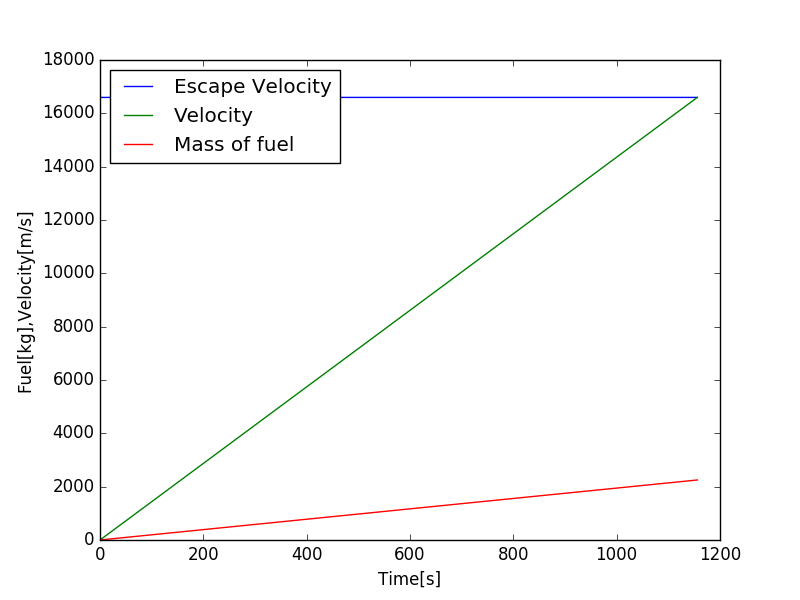
\includegraphics[width = 70mm]{part1launchConstMass.png}
\caption{Shows the mass of fuel increasing has the satellite accelerates. The craft end up using right under 2000 kg of fuel.}
\end{center}
\end{figure}

The plot of the launch with fuel loss shows how the satellite loses fuel as it ascends. The initial fuel was given by equation \ref{eq:Fuel} as $2250.966 kg$.


\begin{figure}[H]
\begin{center}
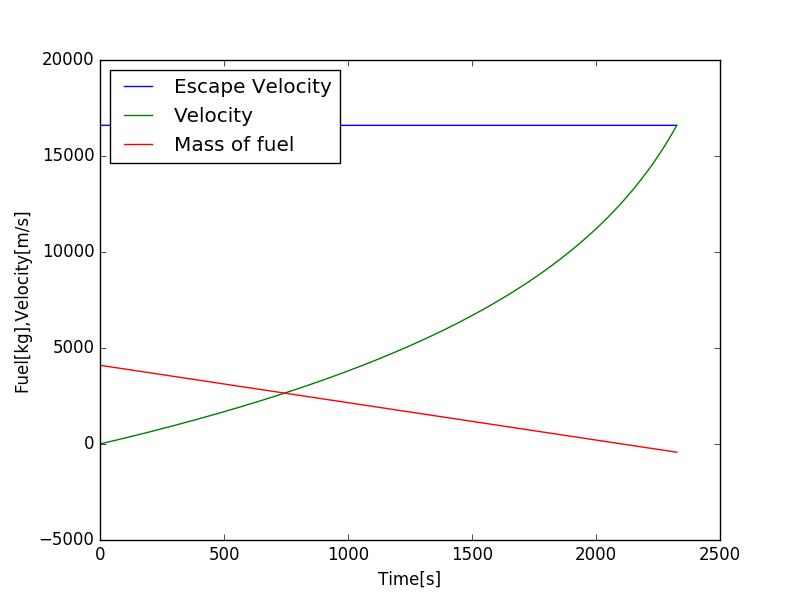
\includegraphics[width = 70mm]{part1launchVarMass.png}
\caption{Shows the mass of fuel slowly going to zeros as the satellite reaches escape velocity.}
\end{center}
\end{figure}

The plot over that as the satellite reaches escape velocity, the mass of the fuel goes to more or less zero. This indicates that my expression for fuel gives the correct amount of fuel.

\subsection{Simulation of out Solar System}
\subsubsection{2-body problem}

The first result is with one planet and the sun. I choose to just look at the largest planet and the sun


\begin{figure}[H]
\begin{center}
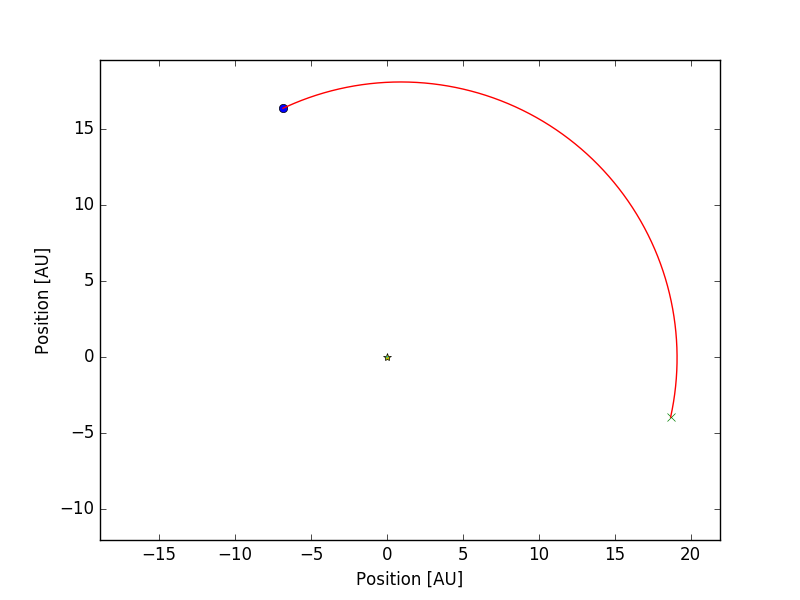
\includegraphics[width = 70mm]{part2onePlanet.png}
\caption{The largest gas giant in the solar system and the sun. Since the planet is quite a distance from the sun, about 16 AU, it only got 1/3 of the way around its orbit during the 20 years.}
\end{center}
\end{figure}

I can see that I have the circular motion I expect, so it passes the rudimentary test for what I expect from planet-sun-system. \\ 

It is more interesting to look at the whole system of 9 planets.

\begin{figure}[H]
\centering
\begin{subfigure}[t]{0.5\textwidth}
\centering
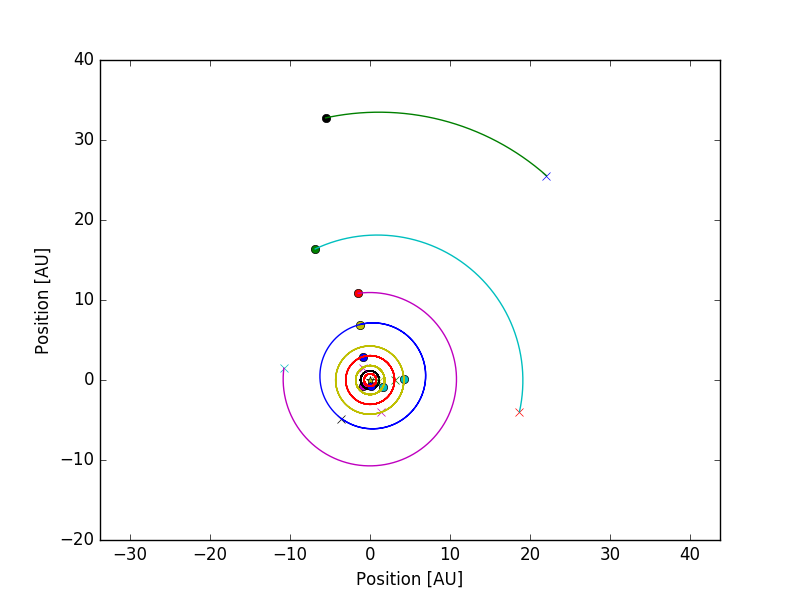
\includegraphics[width=\textwidth]{part2fullSystem.png}
\caption{The orbit of the all 9 planets and the sun. $x$ marks the initial position of the planets, while the ball represents the positions at the end of the simulation.}
\end{subfigure}%
~
\begin{subfigure}[t]{0.5\textwidth}
\centering
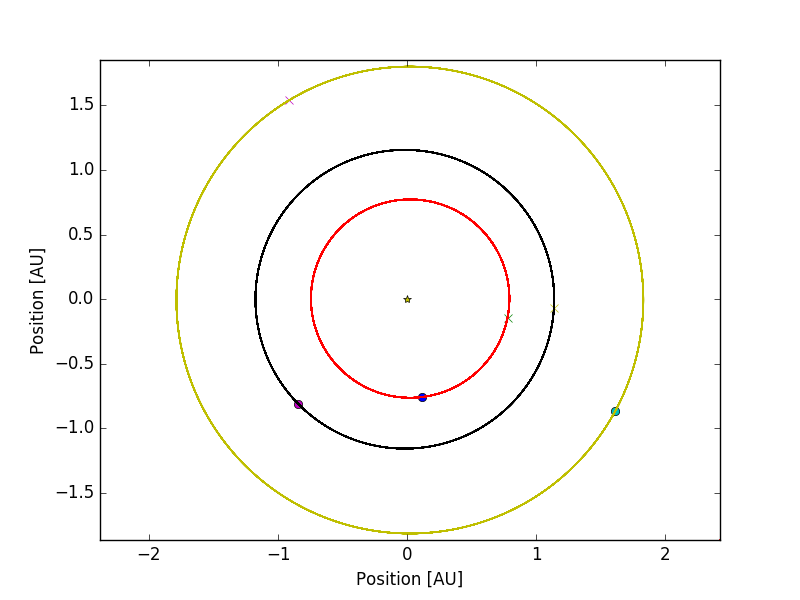
\includegraphics[width=\textwidth]{part2innerPlanets.png}
\caption{A closer look at the inner planets.}
\end{subfigure}%
\end{figure}

I can see that even for the inner planets the simulation seem stable. Since these planets is closer to the sun, they will have orbited more times than the outer planet. There is an error from the numerical method for each orbit, these planets are expected to have accumulated a greater error than the outer planets. Since the I can see that the orbits are stable for the inner planets, I know that the orbits are stable for the rest of the system as Ill.\\

The orbits Ire checked against the analytical solutions, and over the 20 year period, the largest relative error was no more than $0.0036\%$.


\subsubsection{N-body problem}
I am interested in seeing how the other planets influence the sun.

\begin{figure}[H]
\begin{center}
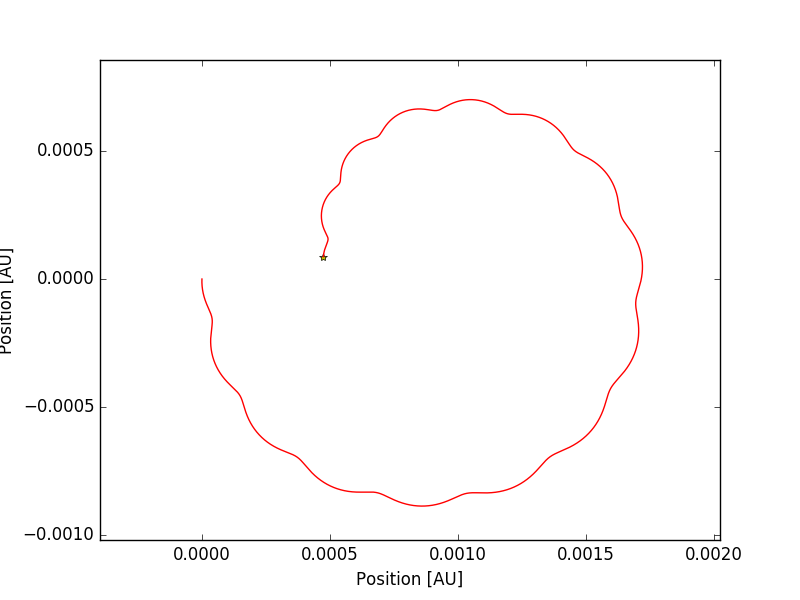
\includegraphics[width = 70mm]{part2posSun.png}
\caption{The motion of the sun. The sun has just finished one orbit of the barycenter of itself and the second largest planet. One can see that this is not a exactly circular orbit, this is because the sun is tugged by the largest planet, which is just 1/4 though its orbit.}
\end{center}
\end{figure}


\begin{figure}[H]
\centering
\begin{subfigure}[t]{0.5\textwidth}
\centering
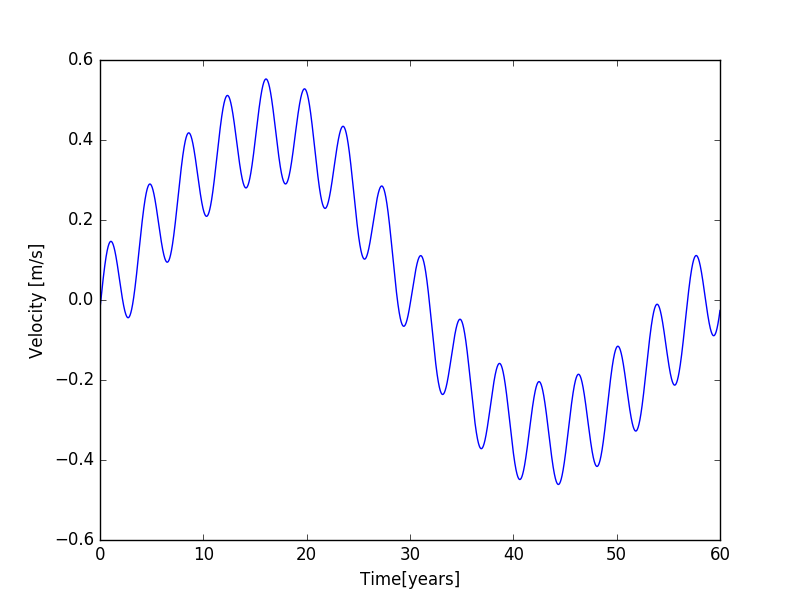
\includegraphics[width=\textwidth]{part2sunNoNoise.png}
\caption{The velocity of the sun towards and away from an observer, gotten from the red shift of the star light.}
\end{subfigure}%
~
\begin{subfigure}[t]{0.5\textwidth}
\centering
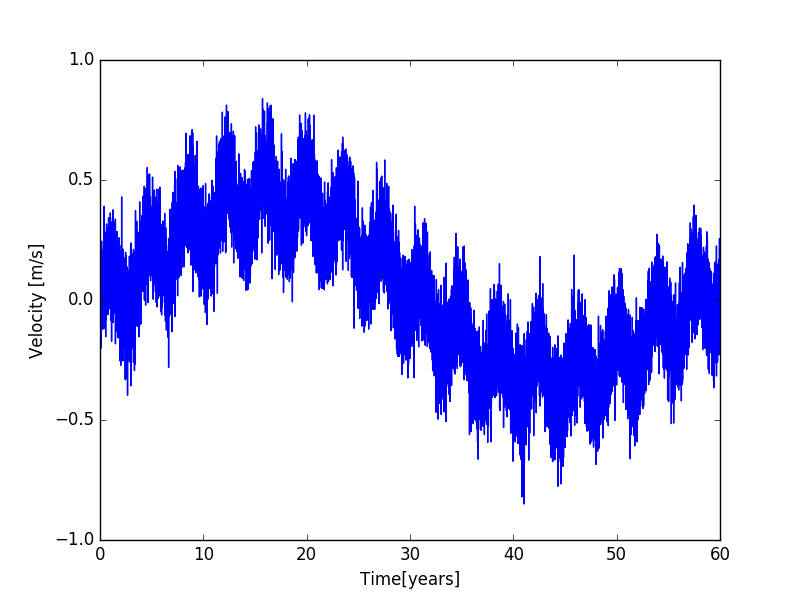
\includegraphics[width=\textwidth]{part2sunNoise.png}
\caption{The velocity of the sun with noise to emulate the noise one gets in real astronomical observations.}
\end{subfigure}%
\end{figure}

I can see that even with noise added to the velocity, the motion is still clearly visible. The difference in velocity is $\pm 0.6 m/s$. With todays technology I am only capable of observing velocity differences of $1 m/s$, meaning that despite there being a clear motion in the data, someone with our technology would not be able to observe it.




\subsection{Information about the planet}
Out star has a temperature of $8284.6 K$, and a radius of $1610671.4 km$. The solar panels I used have an efficiency of $12\%$. Using this and \ref{eq:area} I found that the necessary area of the solar panels to have $40W$ of poIr was   $17.6 m^2$. \\

I know that the habitable zone is the zone in the solar system where $T \in [260,390]$, from \ref{eq:temp} I found the habitable zone to be $r \in [8.1765\cdot 10^8,3.63402\cdot 10^8]$ in $km$. This meant that Isskji, being $6.38 \cdot 10^8 km$ from the sun, was i the middle of the habitable zone.The calculated surface temperature of Isskji is $294.4 K$, a quite comfortable temperature. This was what I had expected after earlier telescope images had shown Isskji to be a garden planet. This gave insured us that Isskji was an interesting planet to explore, in the hope of finding life (the fact that it is our neighbor planet also played a role in the decision.) 

\subsection{Planing the Journey}

The correct angle between the two planets, and therefor the launch, happend after $6.71585$ years.

There was a lot of problems with this part of the simulation. While the algorithm should have worked, the problem, as I knew but didn't take seriously, was that Hohmann transfers and all the associated expressions only work for circular orbits. While the orbits of our home world and Isskji where almost circular, with eccentricity $e = 0.00526$ and $0.00855$, they Ire not completely circular. This meant that the transfers missed. To get an encounter with Isskji I therefor had to adjust $v_0^2$ and $v_{transfer}^2$ ever so slightly, with what in rocket science terminology is called a \textit{fudge factor}. $v_{transfer}^2$ is very sensitive to changes \cite{SpaceDynamics}, so the changes had to be small. Due to an early error in the code, I did not implement that

\begin{align}
v_{transfer}^2 = v_0^2 + v_{transfer}^2
\end{align}  

but

\begin{align}
v_{transfer} = v_0 + v_{transfer}
\end{align} 

This meant that the transfers was even more inaccurate. But after 2 days of tIaking I found that with 

\begin{align}
v_{transfer} = 0.894v_0 + v_{transfer} = 3.525 AU/year
\end{align} 

I where able to get quite close to Isskji. But not close enough. From \ref{eq:safeDist} I find the distance where I could do an orbital injection was $0.000395 AU$. The satellite was not able to get with in this distance after one launcher burn. A correction burn was then hard coded in, to burn when the distance to Isskji was $0.003 AU$. With a correction burn of $0.5 AU/year$, the satellite was able to do an orbital injection. This burn was of size $0.6253 AU/year$. This gave the simulated trip a total $dv$ of $4.65 AU/year$.\\

\begin{figure}[H]
\centering
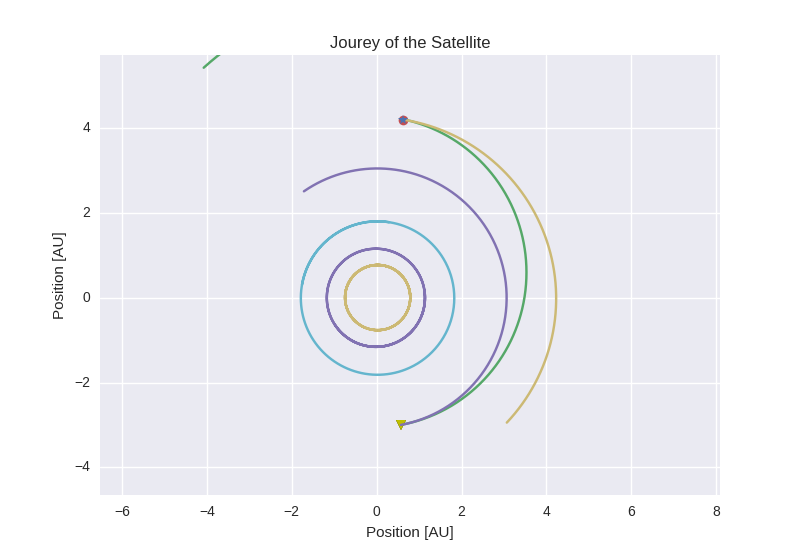
\includegraphics[width = 70mm]{part3SatOrb.png}
\caption{I can see that satellite leaves the home planet and encounters Isskji after almost a half orbit. I can see that the satellite follows the orbit of Isskji, but from this picture it is not clear if it is in orbit.}
\end{figure}

\begin{figure}[H]\label{fig:orbit}
\centering
\begin{subfigure}[t]{0.5\textwidth}
\centering
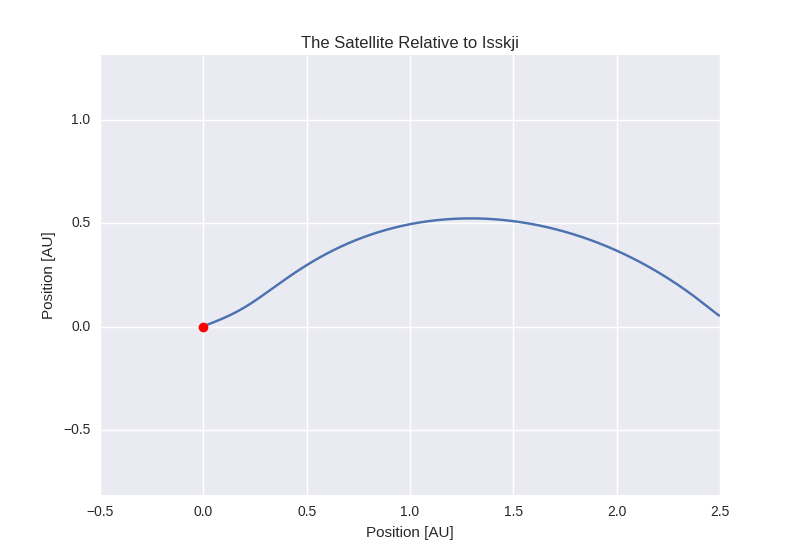
\includegraphics[width=\textwidth]{part3relDist.png}
\caption{The relative distance from the satellite to Isskji}
\end{subfigure}%
~
\begin{subfigure}[t]{0.5\textwidth}
\centering
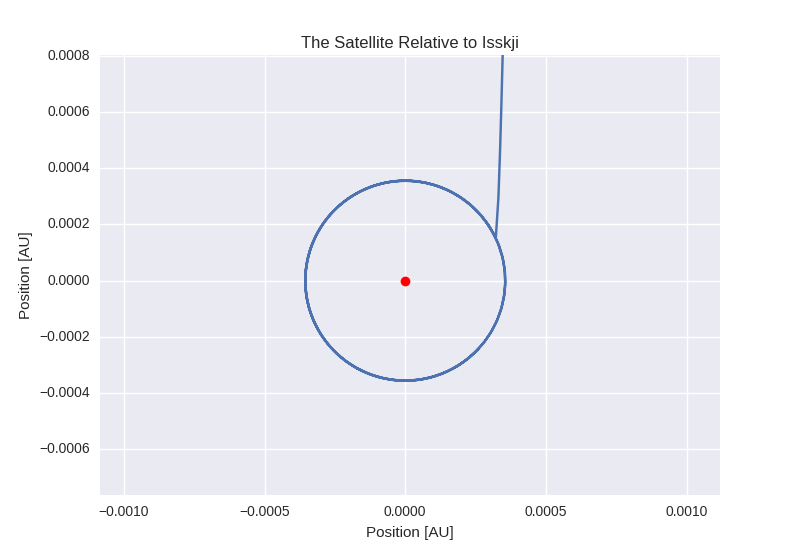
\includegraphics[width=\textwidth]{part3relDistClose.png}
\caption{Same as in (a), but zoomed in to Isskji. I can see that I have a circular orbit.}
\end{subfigure}%
\end{figure}

\ref{fig:orbit} shows that I have simulated a successful journey and orbit around Isskji. It took $2.1$ years.\\

Now I had the total $\Delta v$ for the journey, and could calculate the fuel the satellite needed to reach orbit around Isskji. I decided to bring $10 \%$ extra $\Delta v$. The amount of fuel turned out to be $20558.3 kg$ fuel. 


\subsection{Navigation}

\subsubsection{Velocity}

The reference data when in the rest frame of the star

\begin{tcolorbox}
Reference star 1, at phi = 77.518724 degrees, \\
has delta lambda of  -0.017002884383 nm in the home star rest frame. \\
Reference star 2, at phi = 325.121916 degrees, \\
has delta lambda of   0.017144686369 nm in the home star rest frame. 
\end{tcolorbox}

With this, the algorithm to find the velocity Int fine, without any problems. I tested it against the trivial case where the satellite got the same doppler shifts as in the rest frame, in other words  the satellite is at rest; and where there Ire no doppler shift, the satellite has no relative velocity. The first test shoId $v_{sat} = 0$, and the second gave that $v_{sat} = v_{refstar}$. This shoId that the velocity orientation works.

\subsubsection{Rotation}

There is one problem with this program that became apparent immediately, the pictures have an inverted y-axis. The reason may be that the pictures are made as numpy-arrays. These arrays have the $(0,0)-element$, corresponding to the $(0,0)-pixel$, in the upper left corner, while a picture has its $(0,0)-pixel$ in the loIr left corner. This causes the picture to be upside down. This is easy to correct, but by the time this bug was discovered, the whole starscape atlas was made. This was a lengthy processes, so instead of fixing the bug and remaking the album, I made a function that turn all the incoming pictures upside-down.\\

Then all this is corrected the program finds the correct angle every time.

\begin{figure}[H]
\centering
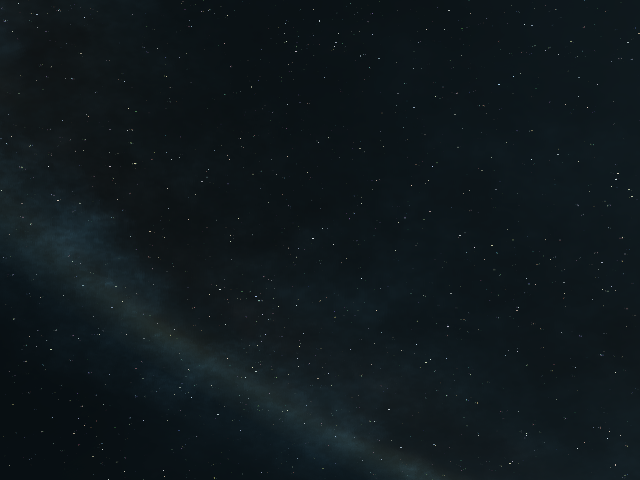
\includegraphics[width = 70mm]{find_orient.png}
\caption{An picture taken by the real satellite used for the first calibration of the orientation software.}
\end{figure}

\subsubsection{Position}

Every thing seemed to work perfectly with this part. I got the correct position on every test and on the orientation on the real satellite. The problem started when I Int through the code while writing this article, the expression for $\partial E / \partial x_i$ was not the one from above \ref{eq:gradient}, but 

\begin{align}\label{eq:gradient}
\frac{\partial E}{\partial x_i} = \frac{8}{N}\sum_{j=1}^N (d_j^{guess} - d_j^{real}){(x_ij^{guess} - x_ij^{planet}}){d_j^{guess}}
\end{align}

When I changed this to real expression, the success rate of this method Int down from $95-100\%$ to $60-90\%$. I do not have a clue why the wrong expression works while \ref{eq:gradient} doesn't. There may be something wrong in our math, so that the "wrong" expression is the correct one, but I do not know. We can also work with the $10-40 \%$ error, we only have to do the gradient descent a with a couple of random guesses and use the most probable result.

\subsection{Simulating the Atmosphere}
\subsubsection{The Mean Molecular Weight of the Atmosphere}


There are 3 sets of pictures I am going to show. The first is the one that looked to fit the model, but had a way to low temperature:

\begin{figure}[H]
\centering
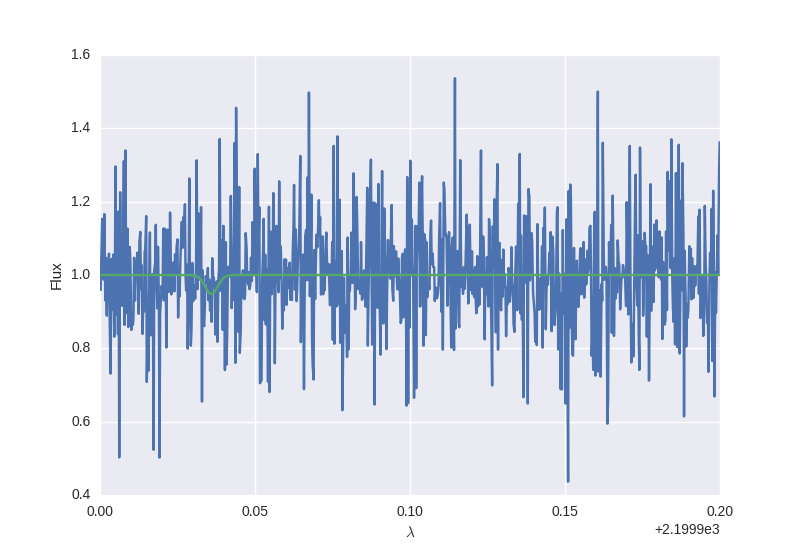
\includegraphics[width = 70mm]{part6wrongTemp2200.png}
\caption{This is $CH_4$, and had a very low temperature $147 K$. If this is a real hit, that we may expect life on Isskji.}
\end{figure}


The next pictures had the same temperature $184.7 K$, but it was lower then expected on our planet.

\begin{figure}[H]
\centering
\begin{subfigure}[t]{0.5\textwidth}
\centering
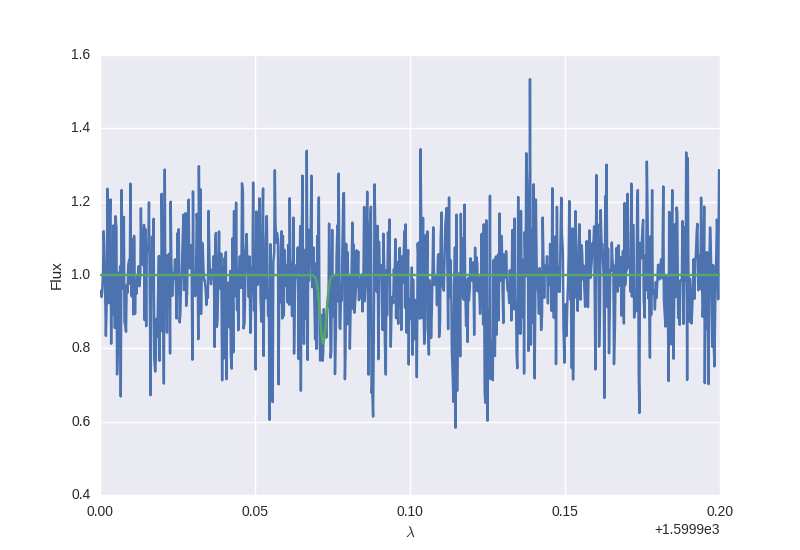
\includegraphics[width=\textwidth]{part6wrongTemp1600.png}
\caption{This gas is $CO_2$.}
\end{subfigure}%
~
\begin{subfigure}[t]{0.5\textwidth}
\centering
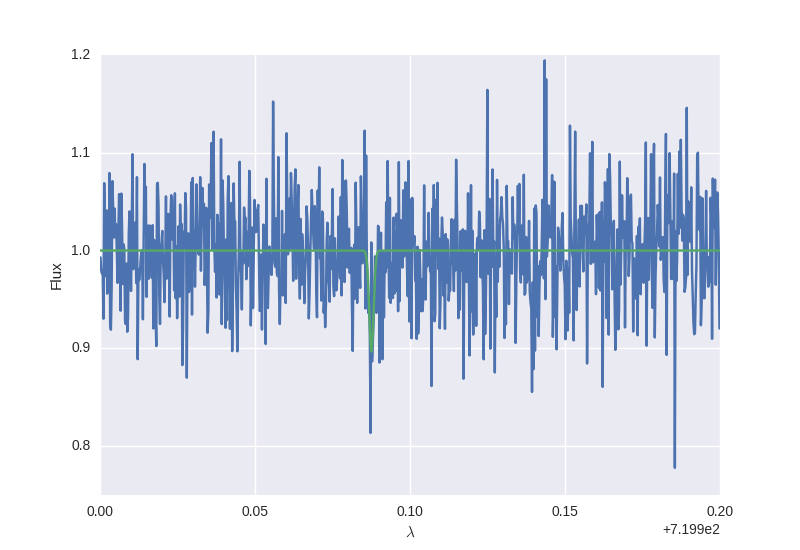
\includegraphics[width=\textwidth]{part6wrongTemp720.png}
\caption{This gas is $H_2O$}
\end{subfigure}%
\end{figure}

The last group also have the same temperature, $271.4$, which is very close to the surface temperature of $294.4 K$

\begin{figure}[H]
\centering
\begin{subfigure}[t]{0.5\textwidth}
\centering
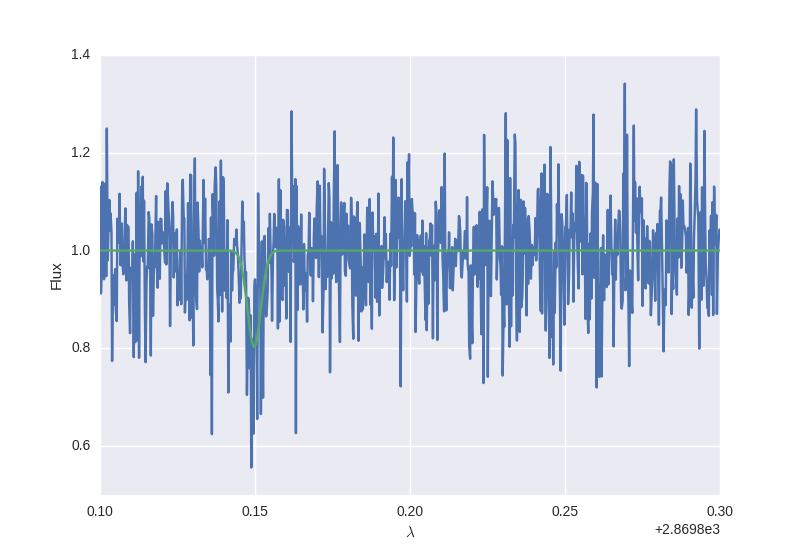
\includegraphics[width=\textwidth]{part6correct2870.png}
\caption{This gas is $N_2O$, which indicates that there might we life on Isskji.}
\end{subfigure}%
~
\begin{subfigure}[t]{0.5\textwidth}
\centering
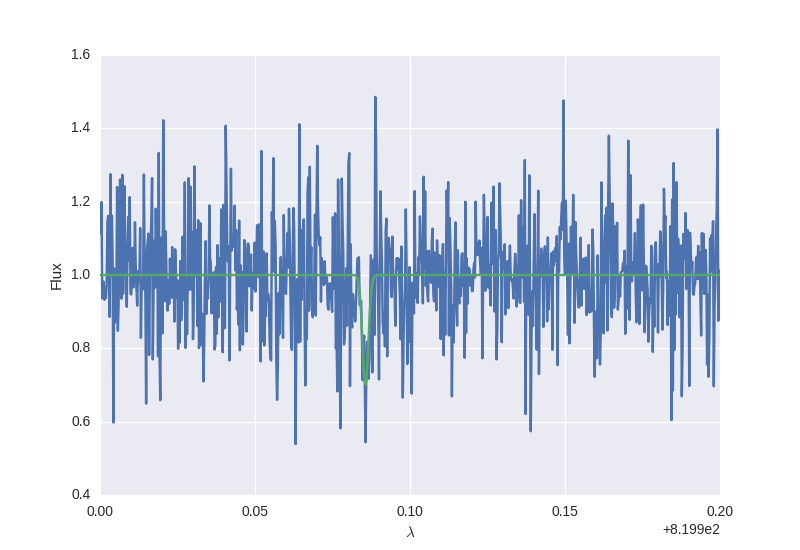
\includegraphics[width=\textwidth]{part6correct820.png}
\caption{This gas is $H_2O$, water. Also important for life.}
\end{subfigure}%
\end{figure}


\textit{I am going to break the fourth wall here!}

There has been a lot of confusion on what the criteria for accepting a gas is. I was not sure if the gases in the atmosphere could have more than one temperature. The first case is quite weak, since the trend is minor. But I was not completely sure if I were to accept the gases at $184.7 K$. If I accepted these and the gases at $294.4 K$ I got a mean molecular weight of $31.013215 u$, and with only the gases at $294.4 K$ I got a weight of $31.01404 u$. Since I accepted 2 extra gases which weighed about the same as those at $294.4 K$, the mean changed only slightly. \\

For the rest of the simulations I went with $\mu = 31.01404 u$\\

It is possible to do this minimization with a gradient descent, but I found this to be much slower so I ended up using the "random sample" method  

\subsubsection{The Atmosphere}

\begin{figure}[H]
\centering
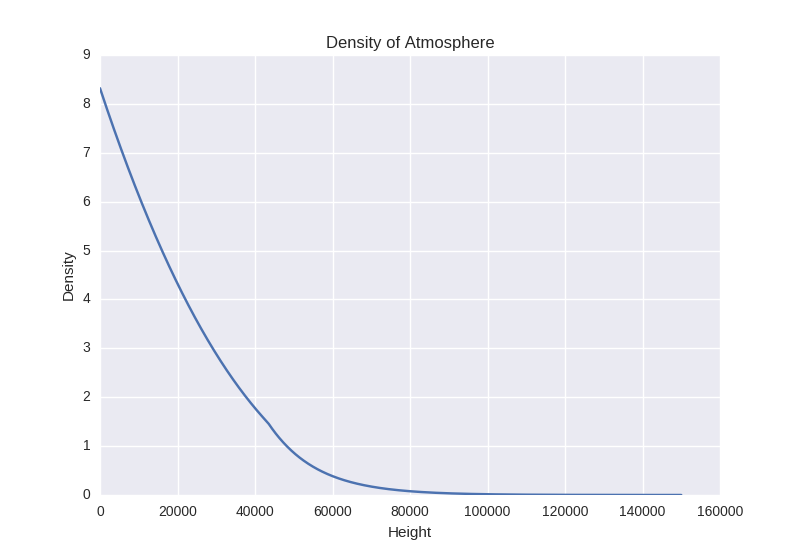
\includegraphics[width = 70mm]{part6atmos.png}
\caption{The density of the atmosphere as a function of hight over the surface.}
\end{figure}

We can see that the adiabatic density decreases fast. Near $40 km$ the atmosphere becomes isothermal, and the decrease of the density begins to go slower. Since the atmosphere is found using an analytical expression, there are few things that went wrong the simulation.

\subsection{Landing}
\subsubsection{Low orbit}
As will be describes below, the Hohmann transfer to get to low orbit in the simulation did not correspond well with reality, so I had to update the position in the simulation to ensure a correct, circular low orbit.\\

The atmosphere of Isskji is quite thick, with $\rho_0 \approx 8$, this means that the safe distance for a stable low orbit is $390 km$, which is quite high compared with earth where a low orbit occurs at $160 km$ above the surface.\\

\begin{figure}[H]
\centering
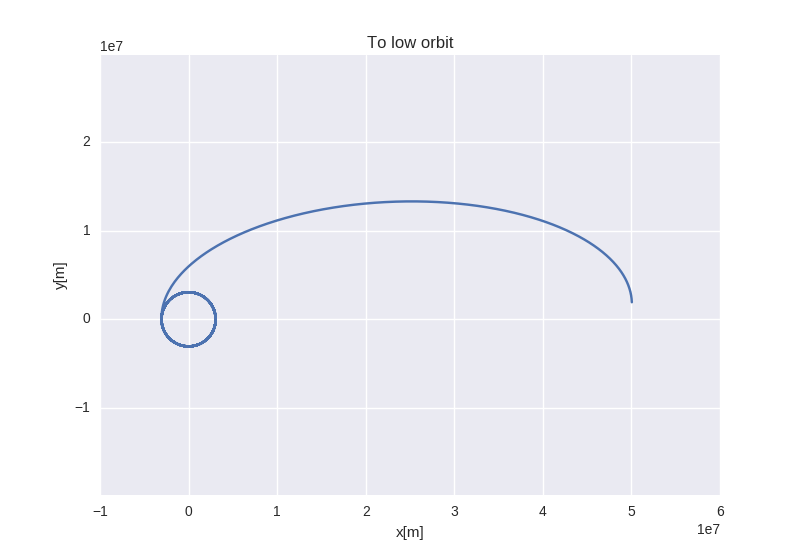
\includegraphics[width = 70mm]{part6orb.png}
\caption{Shows the Hohmann transfer from high to low orbit.}
\end{figure}

In its equatorial orbit at $390 km$ 20 pictures were planed out to look for a suitable landing site.


I could have orbited the planet in an polar orbit if I wanted to find a better place to land. In an polar orbit I would wave been able to take pictures of the whole surface. The reason I chose not to go into polar orbit was simply time constrains.

\subsubsection{The Landing}
Since the acceleration inside the atmosphere is dependent on velocity, leapfrog may be unstable. This is because the velocity is in between steps. But after some trial it seemed that this didn't have so much to say, and I went with a normal leapfrog.\\
 
The height to which I had to do a Hohmann transfer was found, by trial and error, to be $290 km$ below the current orbit. This gave me a nice half orbit before landing:

\begin{figure}[H]
\centering
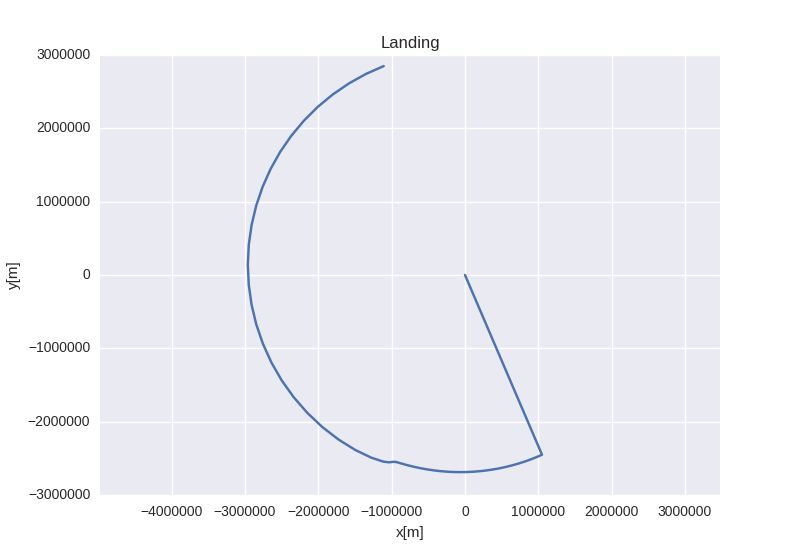
\includegraphics[width = 70mm]{part7landing.png}
\caption{Shows the half orbit before hitting the ground. The simulation was stopped when hitting the surface, but due to a bug where the last positions in the array is not filled, and thus only contains zeros, it looks like the lander continues to the center of the planet.}
\end{figure}

And after more trail and error I found that if I let the satellite loiter in orbit for $40950 sec$ after entering the low orbit, before launching the lander. The simulation then gave me the information

\begin{tcolorbox}
You landed at time 145815 with velocity -2.93852\\
ParachuteSize:  7.64794319168\\
Landing Angle:  92.002628546\\
Landing Angle in Rad:  1.60574878862
\end{tcolorbox}

The goal was $96.97^\circ$(see below) (being in an equatorial orbit $\theta$ is always $180^\circ$). The simulation said I landed at $96.24^\circ$, which I found satisfactory, and decided to go for it.

My thought was that the simulation of through the atmosphere would be unstable, and that I had to use very small $\Delta t$, but after some trail, it seemed that it needed only the same $\Delta t$ as for the normal orbit $0.1$.

\subsubsection{A Safe Landing}
As we have seen Isskjis atmosphere is quite thick, $\rho_0 \approx 8$, so I didn't expect that the size of the parachute had to be very large to reach a safe landing velocity of $3m/s$. This turned out to be correct: the parachute need only be  $7.65 m^2$, which is smaller than a standard skydiving parachute.


\subsection{Launching the Real Satellite} 
Then it was time to launch the satellite for real. We waited $6.72$ years and launched. The launch was the same as in the simulation. I asked the satellite to orient it self after 1 and 2 years. The first orientation was the calibration orientation, and went without any hitch. Both orientations showed the satellite to be a little of course, but not by very much. 

\begin{tcolorbox}
Orient 2:\\
Expected Position: [ 1.07228774  4.08232315]\\
Real Position: [1.07602195366 , 4.0834412672]
\end{tcolorbox}

This was so close that no correction burn was done yet. When the satellite came close to the point of the correction burn, it got the command to do multiple orientations. When the point closest to Isskji was found after $2.05$ years, I decided to do the correction burn, even though it wasn't the same place it the simulation. It was only as small burn $(-0.49152321, 0.26571668)$. One and a half days later the satellite was inside the safe distance from Isskji and was able to do an injection burn of $(0.11537089, -0.32227829)$. The total $\Delta v$ needed on the real journey was $3.145 AU/year$, which is lower than the expected $\Delta v$ from the simulations.\\

Now that the satellite was in orbit it was time to get into a lower orbit. The satellite was asked to orientate right after it had circularized the low orbit. This orientation was somewhat off. The simulation was therefor forced to start at this point, and then circularize again. This time the it worked and the satellite showed a stable low circle orbit.\\

In its equatorial orbit at $390 km$ 20 pictures were taken, between $ 90461-107461 sec$, to find a suitable landing site. Four are shown here (due to the fact that 20 pictures would take a lot of space).

\begin{figure}[H]
\centering
\begin{subfigure}[t]{0.5\textwidth}
\centering
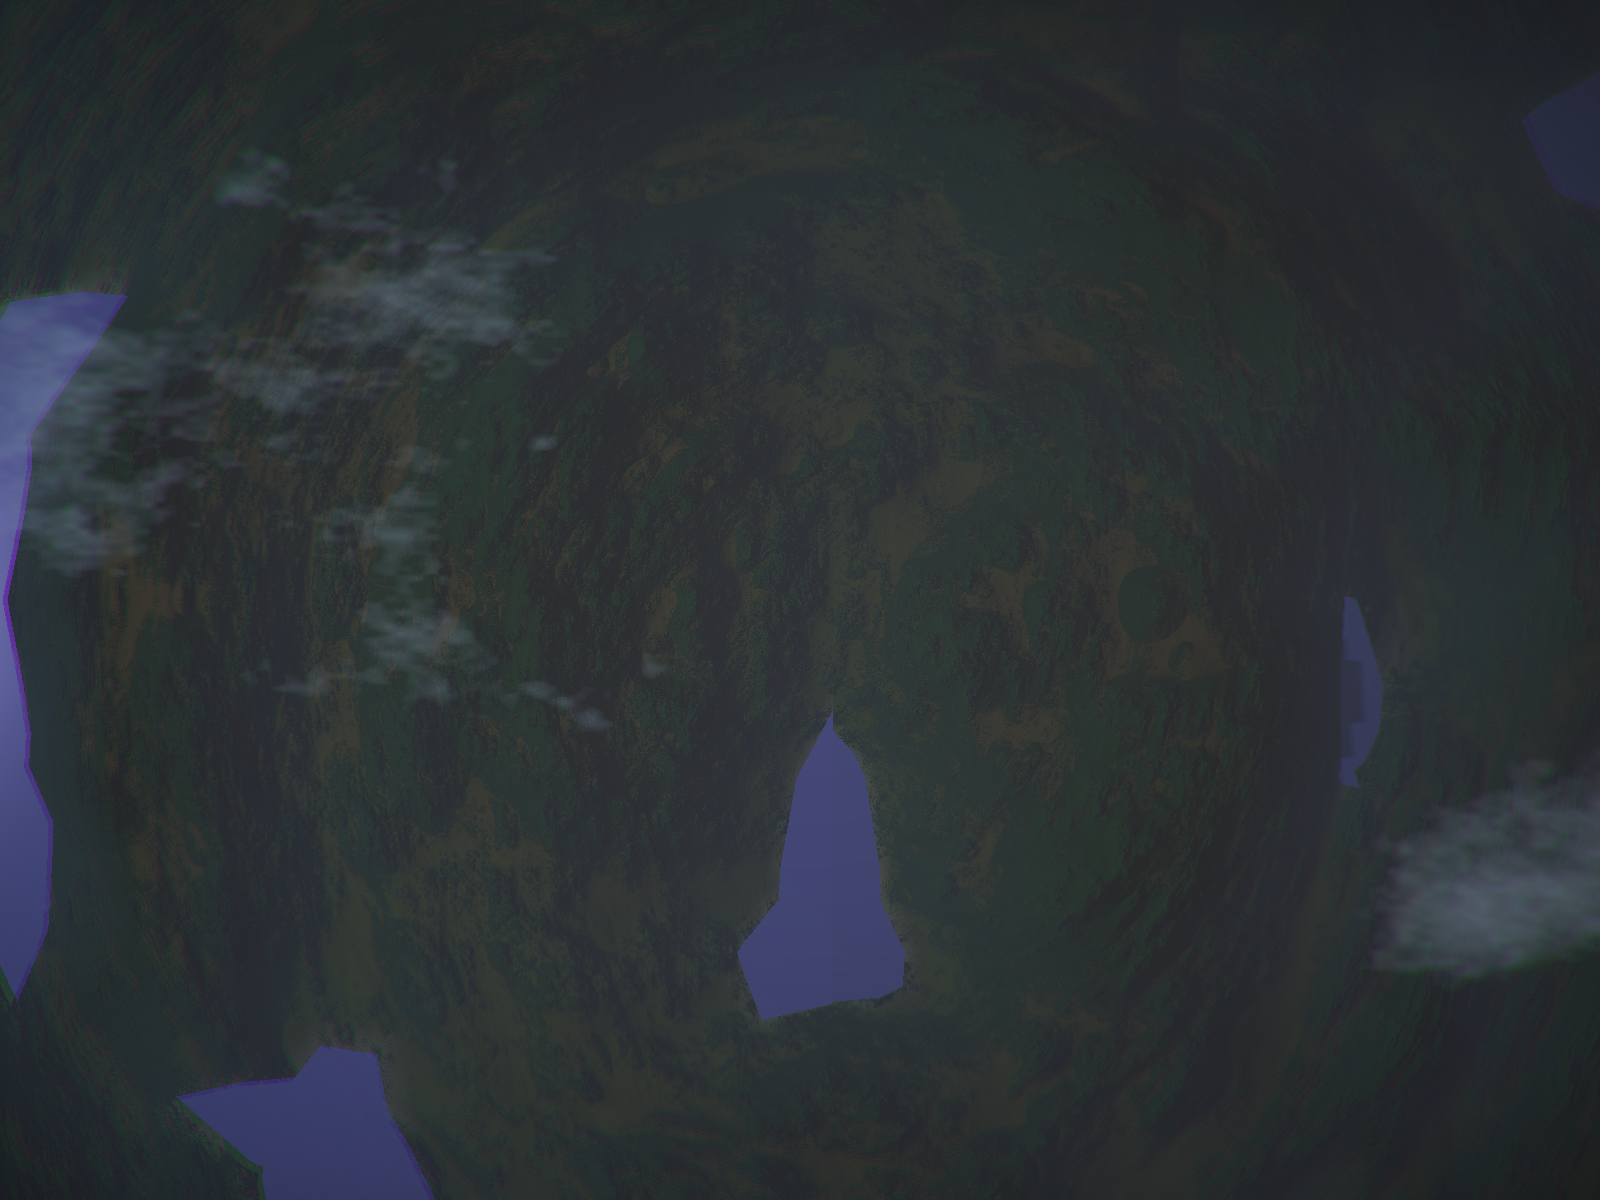
\includegraphics[width=\textwidth]{Image0005.png}
\end{subfigure}%
~
\begin{subfigure}[t]{0.5\textwidth}
\centering
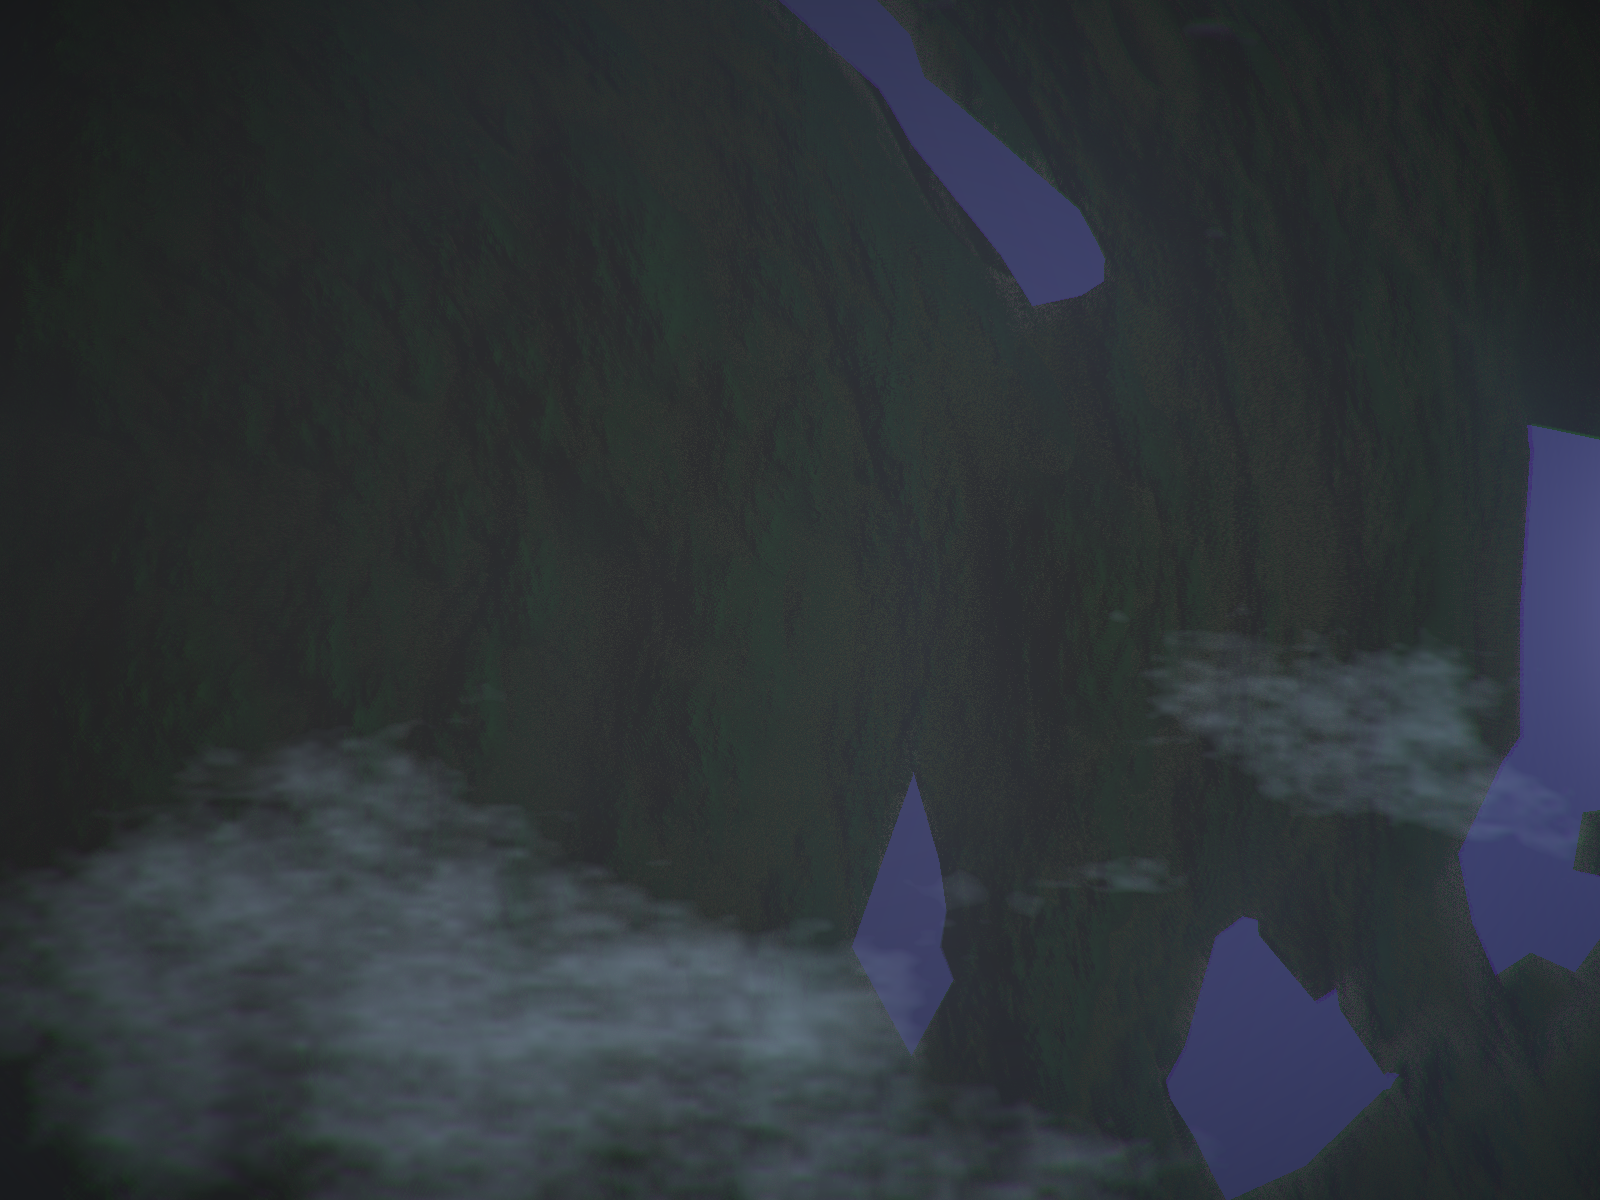
\includegraphics[width=\textwidth]{Image0006.png}
\end{subfigure}%
\quad
\begin{subfigure}[t]{0.5\textwidth}
\centering
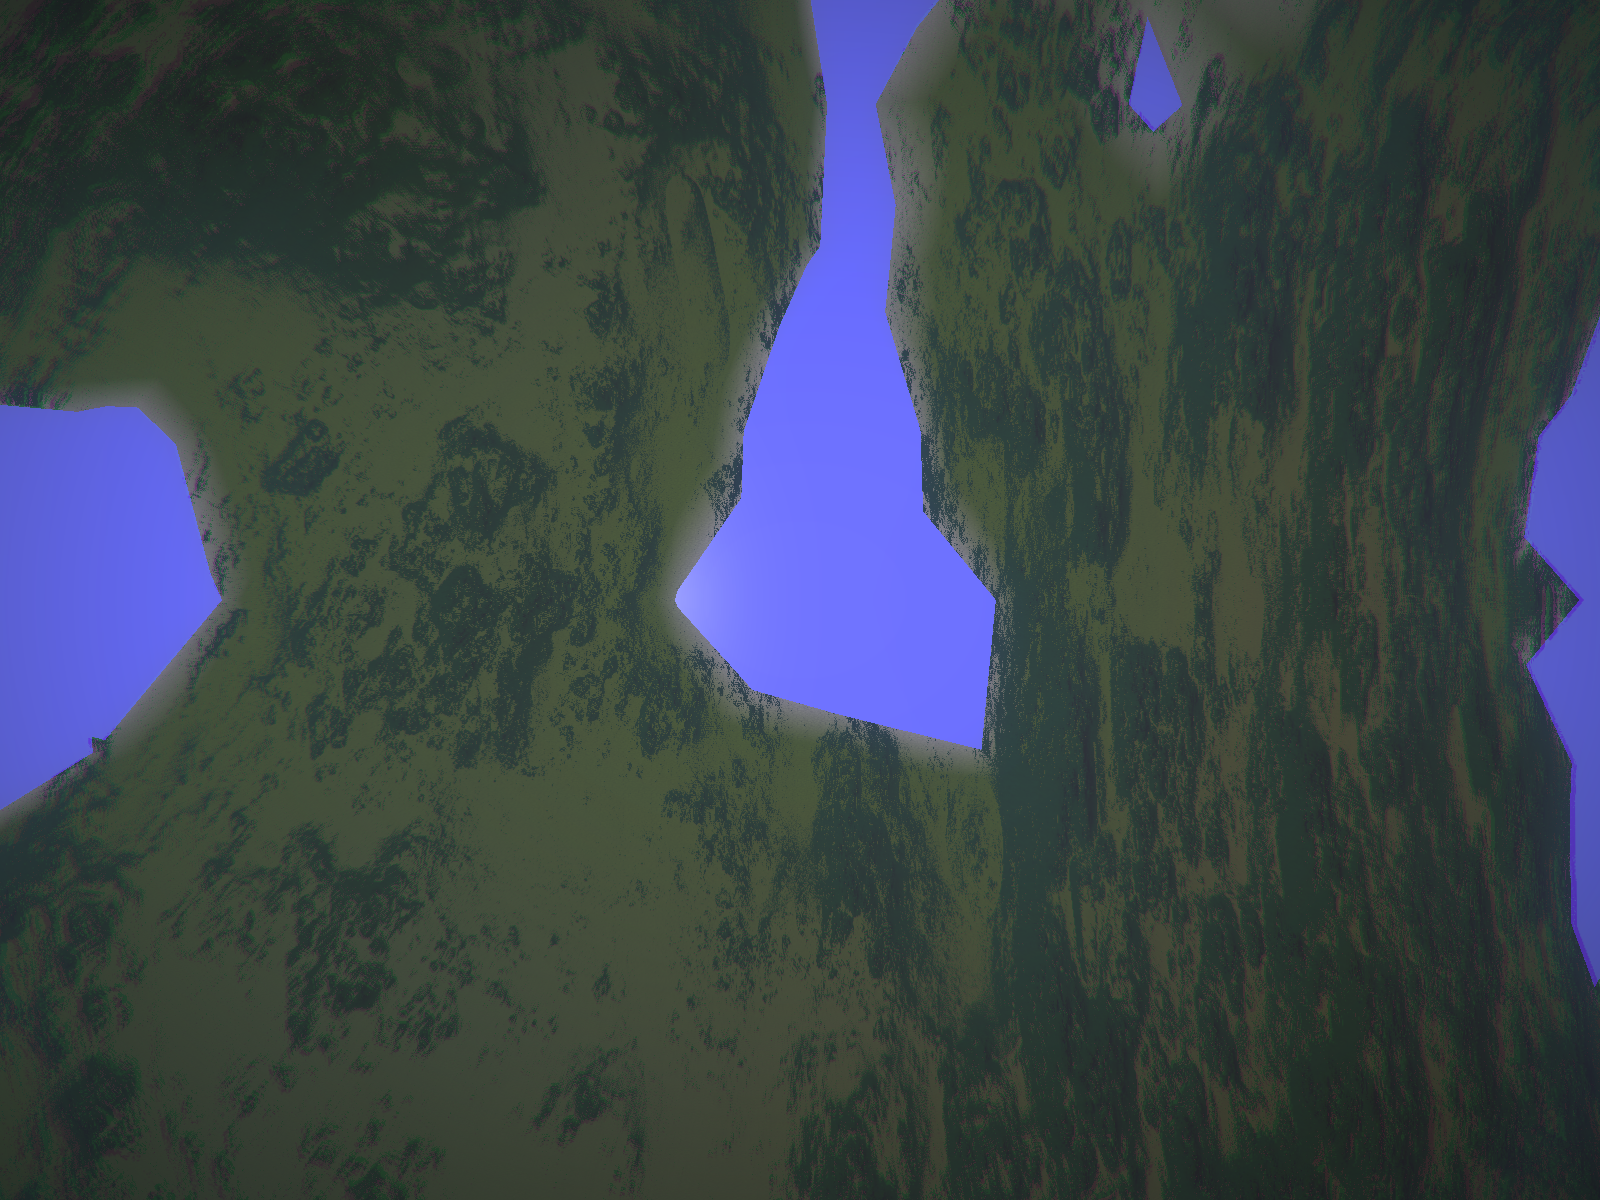
\includegraphics[width=\textwidth]{Image0007.png}
\end{subfigure}%
~
\begin{subfigure}[t]{0.5\textwidth}
\centering
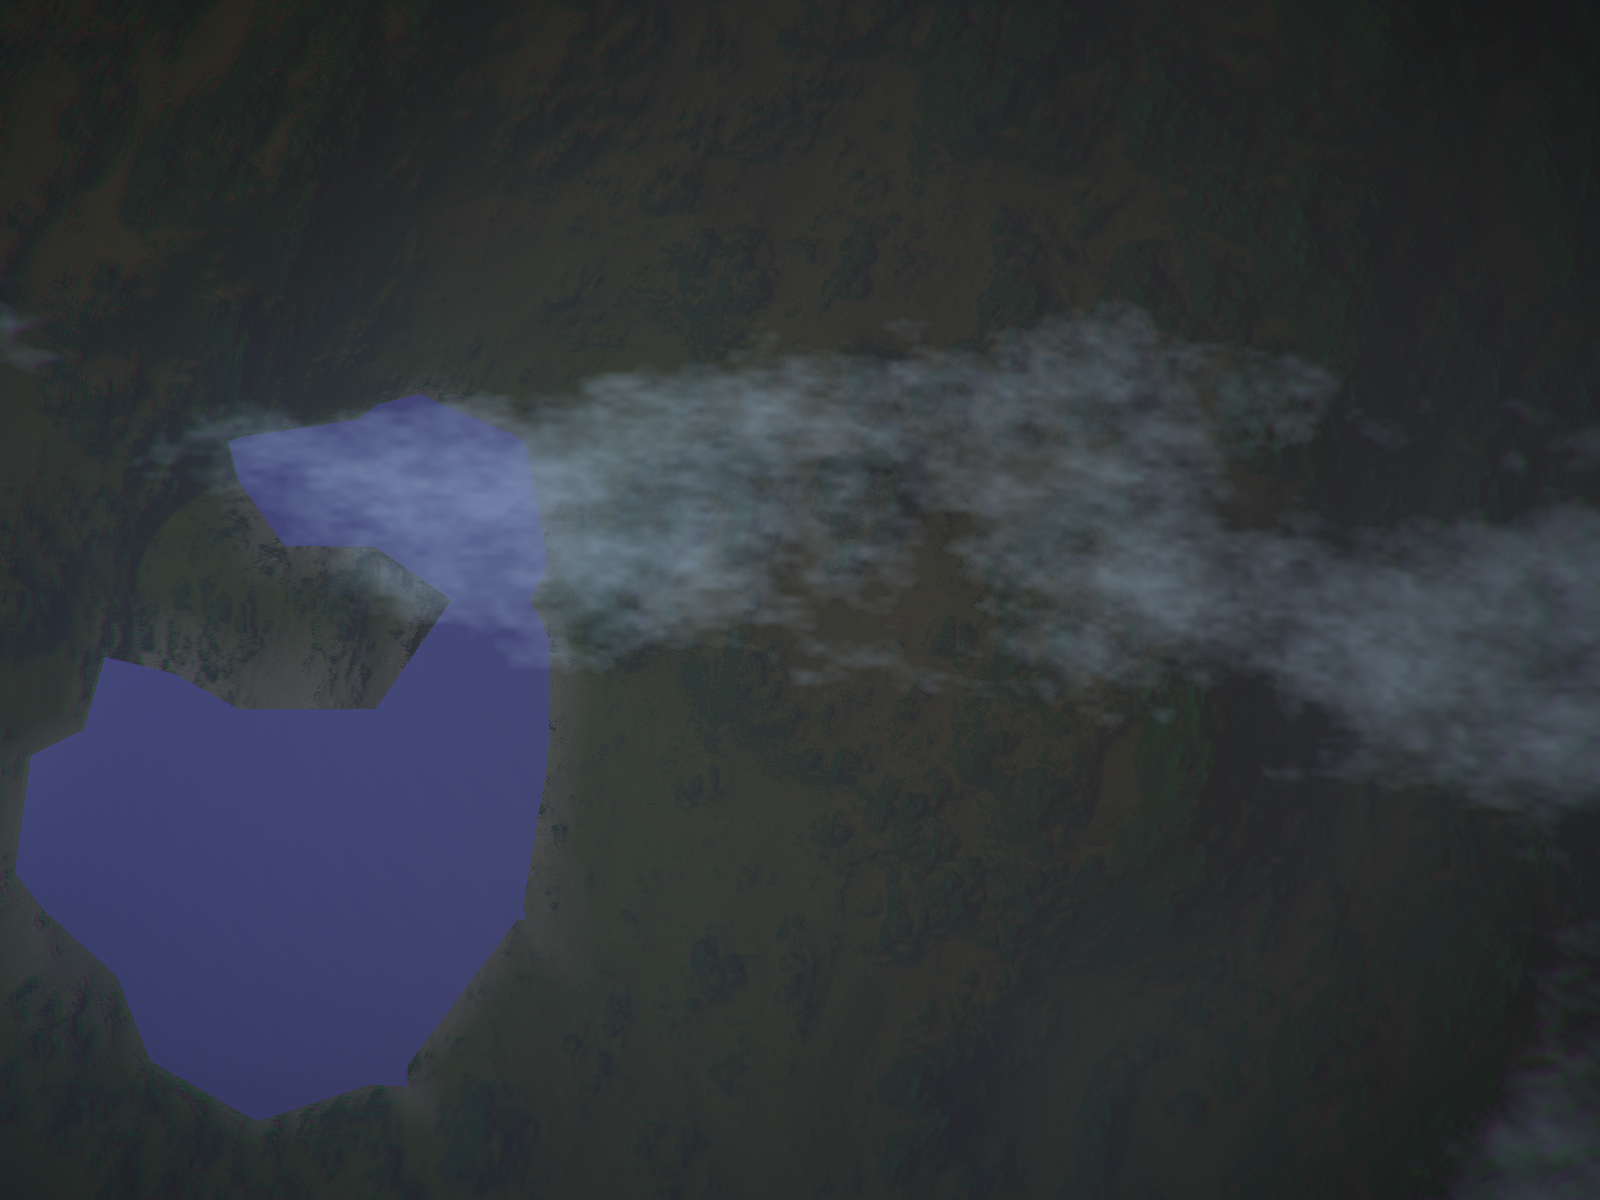
\includegraphics[width=\textwidth]{Image0008.png}
\end{subfigure}%
\caption{Pictures of the surface taken over a couple of orbits.(The subplots are mushed together because a couldn't find a way to make a good looking figure with 4 subfigures...)}
\end{figure}


Neither in these nor the rest of the pictures showed any place that sticks out. But I chose to land at the site showed in the upper left picture, due to the small lake surrounded by, what looks like, two mountains. I found that the local coordinates were $(180^\circ , 96.97^\circ)$. \\

After waiting the $40950 sec$, the lander was launched, and the whole control room was deadly silent in the wait for the lander to make contact after landing. And then this message was received:

\begin{tcolorbox}
Successful landing! Landed on planet nr 1 at time 145361 s with velocity 2.99479 m/s. Congratulations! \\
Landing site: phi =  93.8127183984 deg,  theta =  90.0 deg.
\end{tcolorbox}

And the control room exploded in ecstasy! My planned landing site was $96.97^\circ$, my simulated landing site was $96.24^\circ$ and the real landing site was at $93.81^\circ$. And the lander had landed just under $3 m/s$ without any need for landing boosters. The mission seemed to be a huge success! \\

But then the landing video came back, and the landing site looked nothing like the picture. The simulation and the real landers coordinates matched well, so the mistake must have happened when converting the picture in to the local coordinate on the surface. I looked carefully though the code, but I could not find the mistake. We were so close to total success!  



\section{Appendix A: Numerical Methods}
\subsection{Leapfrog}\label{sec:leap}

Leap frog is a method for integrating functions with a known starting point, of the form \cite{leap} 

\begin{align}
\frac{dx}{dt} = F(x)
\end{align}

The algorithm goes like

$$
x_i = x_{i-1} + v_{i-1/2}\Delta t
$$

$$
a_i = F(x_i)
$$

$$
v_{i+1/2} = v_{i-1/2} + a_i \Delta t
$$

An easier way of implementing this is by the algorithm

\begin{enumerate}
\item Update $v_{i+1/2} = v_{i} + 0.5a_i \Delta t$
\item Loop over doing a normal forward Euler.
\end{enumerate}

Leap frog is of seconds order \cite{leap2}. But the strength of leapfrog is that it is suited for dynamical system. It conserves energy well in oscillating system. It may not conserve energy during an oscillation, but it is conserved between oscillations. \\

Implemented as stated above, the leapfrog is as fast as Euler-Cromer. 
\subsection{Gradient descend}\label{sec:gradient}

Gradient descent is a numerical method for minimizing an error function. The error function in our problem is

\begin{align}
E(x_1,x_2) = \sum_{j=1}^N(d_j^{guess} - d_j^{real})^2
\end{align} 

where 

\begin{align}
d_j^{guess} = \sqrt{(x_1^{guess}-x_1^{planet}) + (x_2^{guess}-x_2^{planet})}
\end{align}

$E(x_1,x_2)$ makes up a potential surface, and we are interested in finding the global minimum of this surface. We know that the gradient $\nabla E(x_1,x_2)$ at a point is a vector that point towards a maximum. Knowing that it is easy to see that if we go a small in the opposite direction of the gradient in that point, we will go towards the minimum. This is the idea behind gradient descent. The algorithm is

\begin{enumerate}
\item Start with a guess.
\item Loop over a fixed number of steps (I used $10^{5}$)
\item Update the guess' coordinate $x_i$ with $\omega \frac{\partial E}{\partial x_i}$ for each step.
\end{enumerate}

Where $\frac{\partial E}{\partial x_i}$ is the error function differentiated for $x_i$

\begin{align}\label{eq:gradient}
\frac{\partial E}{\partial x_i} = \frac{2}{N}\sum_{j=1}^N (d_j^{guess} - d_j^{real})\frac{(x_ij^{guess} - x_ij^{planet}}{d_j^{guess}})
\end{align}

the weight $\omega$ is important. If $\frac{\partial E}{\partial x_i}$ is larger than the width of the well of the minimum, we are going to climb out of this well, and we may end up diverging instead of  covering. Because of this we multiply $\frac{\partial E}{\partial x_i}$ by some $\omega < 1$ to keep $\frac{\partial E}{\partial x_i}$ smaller than the well.\\

The problem with gradient descent is that it doesn't only find global minimums, but also local ones. This may be the case with our error function, but these are so large that the gradient descent more often finds the global.

\section{Appendix B: Fuel Equation}\label{sec:Fuel}

To find an analytical expression for the fuel use, I am going to derive the rocket equation using the parameters I get from out engine. I am going to start with Newton's 2. law to find the acceleration for our system:

\begin{equation}
a = \frac{F}{m} = \frac{F_b n_b}{m_f(t) + m_l} 
\end{equation}

Since the system are losing mass:

\begin{equation}
a = \frac{F_b n_b}{(m_{f0} - n_b m_e t) + m_l} = \frac{F_b n_b}{(m_{f0} - \Delta m t) + m_l}
\end{equation} 

Where $m_{f0}$ is the initial mass of the fuel, and $\Delta m$ is the mass loss per second. I separate the variables and solve the differential equation:

\begin{equation}
v(t) = \int \frac{F_b n_b}{(m_{f0} - \Delta m t) + m_l} dt
= K - \frac{F_b}{m_e} \ln(m_{tot} - \Delta m t) 
\end{equation}

Where $m_{tot} = m_l + m_{f0}$. Using the boundary expression I find

\begin{equation}
K = v_0 + \frac{F_b}{m_e} \ln (m_{tot})
\end{equation}

This gives us the rocket equation for our satellite: 

\begin{equation}
v(t) =v_0 + \frac{F_b}{m_e} \ln \left(\frac{m_{tot}}{m_{tot} - \Delta m t} \right)
\end{equation}

I can see that $\frac{F_b}{m_e}$ has the dimension of velocity. This expression corresponds to the velocity of particles escaping (exhaust velocity). If I call this $v_e$ I have the original rocket equation. I want to have use all the fuel when the desired $\Delta v$ i reached. The only mass left then is the mass of the satellite, so $m_{tot} - \Delta m t = m_l$. From this I can find the equation for fuel needed:

\begin{equation}
m_{f0} = m_l(e^{\frac{\Delta v m_e}{F_b}} - 1)
\end{equation}


\section{Appendix C: The Expression for the Atmosphere}\label{sec:atmosphere}
\subsection{The isothermal atmosphere}
To find the analytical expression for the isothermal part of atmosphere I start with the equations for an ideal gas \cite{1e}

\begin{align}\label{eq:idealgas}
P = \frac{\rho kT}{\mu m_H}
\end{align}

and for hydrostatic equilibrium 

\begin{align}\label{eq:hydrostatic}
\frac{dP}{dr} = -\rho \frac{GM(r)}{r^2}
\end{align}

I am going to make the approximation that the gravitational acceleration is the same in the whole atmosphere:

\begin{align}
\frac{GM(r)}{r^2} = g_r
\end{align}

I solve \ref{eq:idealgas} for $\rho$ and sat it in to \ref{eq:hydrostatic}, I get that

\begin{align}
\frac{dP}{dr} = -Pg h_0
\end{align}

\begin{align}
h_0 = \frac{kT}{m_H g \mu}
\end{align}

This differential equation can easily be solved by separating variables, and I get that

\begin{align}
P(h) = C e^{-\frac{h}{h_0}} = P_0 e^{-\frac{h}{h_0}}
\end{align}

And using this in the ideal gas law I find

\begin{align}
\rho (h) = \frac{P_0}{h_0} e^{-\frac{h}{h_0}} = \rho_0 e^{-\frac{h}{h_0}}
\end{align}

\subsection{The adiabatic atmosphere}
Including equations \ref{eq:idealgas} and \ref{eq:hydrostatic} there is one more equation for an adiabatic system

\begin{align}\label{eq:abiabatic}
P^{1-\gamma}T^{\gamma} = constant
\end{align}

$\gamma = 1.4$. This constant is not known but by differentiating the expression we can get rid of it (this first step was inspired by \cite{adia}, but the rest was done by us)

\begin{align}
\frac{d}{dh}(P^{1-\gamma}T^{\gamma}) = \frac{dP}{dh}(1-\gamma)\left(\frac{T}{P} \right)^{\gamma} + \frac{dT}{dh}\gamma \left(\frac{T}{P} \right)^{\gamma-1} = 0
\end{align}

\begin{align}
\Rightarrow \frac{dP}{P} = \frac{\gamma}{\gamma - 1}\frac{dT}{T}
\end{align}

rewriting the hydrostatic equilibrium we get that

\begin{align}
\frac{dP}{P} = -(g h_0) dh = \frac{\gamma}{\gamma - 1}\frac{dT}{T}
\end{align}

And solving this differential equation gives us the temperature

\begin{align}
T(h) = -g h_0 \frac{\gamma-1}{\gamma}h + C
\end{align}

$T(0) = C = T_0$

\begin{align}\label{eq:adiatemp}
T(h) = T_0 \left( 1 -\frac{\gamma - 1}{\gamma} \frac{h}{h_0} \right)
\end{align}

Setting this back into \ref{eq:abiabatic} we get that

\begin{align}
P(h) = cT(h)^{\frac{\gamma}{\gamma-1}} = cT_0 \left( 1 -\frac{\gamma - 1}{\gamma} \frac{h}{h_0} \right)^{\frac{\gamma}{\gamma-1}} = P_0\left( 1 -\frac{\gamma - 1}{\gamma} \frac{h}{h_0} \right)^{\frac{\gamma}{\gamma-1}}
\end{align}

Now using the ideal gas law we get that

\begin{align}
\rho (h) = \frac{P(h)}{T(h)}\frac{\mu m_H}{k} = \frac{P_0}{T_0}\frac{\mu m_H}{k}\left( 1 -\frac{\gamma - 1}{\gamma} \frac{h}{h_0} \right)^{\frac{\gamma}{\gamma-1} - 1}
\end{align}

\begin{align}\label{eq:adiadens}
\rho (h) = \rho_0 \left(1-\frac{\gamma - 1}{\gamma} \frac{h}{h_0}\right)^{\frac{1}{\gamma - 1}}
\end{align}

\subsection{The boundary}
I was interested in finding $\rho_0$ for the isothermal atmosphere, which is the pressure at the height where $T(h) = T_0/2$. If I use \ref{eq:adiatemp} with  $T(h) = T_0/2$ and solve for $h$, I found that this hight is

\begin{align}
h_{boundary} = \frac{\gamma}{2(\gamma -1)}h_o
\end{align}

and using this in \ref{eq:adiadens} I got that 

\begin{align}
\rho_0^{isothermal} = \rho(h_{boundary}) = \rho_0 \left(\frac{1}{2} \right) ^{\frac{1}{\gamma +1}}
\end{align}


\bibliography{ref} 
\bibliographystyle{plain}






\end{document}